%% fcup-thesis.tex -- document template for PhD theses at FCUP
%%
%% Copyright (c) 2015 João Faria <joao.faria@astro.up.pt>
%%
%% This work may be distributed and/or modified under the conditions of
%% the LaTeX Project Public License, either version 1.3c of this license
%% or (at your option) any later version.
%% The latest version of this license is in
%%     http://www.latex-project.org/lppl.txt
%% and version 1.3c or later is part of all distributions of LaTeX
%% version 2005/12/01 or later.
%%
%% This work has the LPPL maintenance status "maintained".
%%
%% The Current Maintainer of this work is
%% João Faria <joao.faria@astro.up.pt>.
%%
%% This work consists of the files listed in the accompanying README.

%% SUMMARY OF FEATURES:
%%
%% All environments, commands, and options provided by the `ut-thesis'
%% class will be described below, at the point where they should appear
%% in the document.  See the file `ut-thesis.cls' for more details.
%%
%% To explicitly set the pagestyle of any blank page inserted with
%% \cleardoublepage, use one of \clearemptydoublepage,
%% \clearplaindoublepage, \clearthesisdoublepage, or
%% \clearstandarddoublepage (to use the style currently in effect).
%%
%% For single-spaced quotes or quotations, use the `longquote' and
%% `longquotation' environments.


%%%%%%%%%%%%         PREAMBLE         %%%%%%%%%%%%

%%  - Default settings format a final copy (single-sided, normal
%%    margins, one-and-a-half-spaced with single-spaced notes).
%%  - For a rough copy (double-sided, normal margins, double-spaced,
%%    with the word "DRAFT" printed at each corner of every page), use
%%    the `draft' option.
%%  - The default global line spacing can be changed with one of the
%%    options `singlespaced', `onehalfspaced', or `doublespaced'.
%%  - Footnotes and marginal notes are all single-spaced by default, but
%%    can be made to have the same spacing as the rest of the document
%%    by using the option `standardspacednotes'.
%%  - The size of the margins can be changed with one of the options:
%%     . `narrowmargins' (1 1/4" left, 3/4" others),
%%     . `normalmargins' (1 1/4" left, 1" others),
%%     . `widemargins' (1 1/4" all),
%%     . `extrawidemargins' (1 1/2" all).
%%  - The pagestyle of "cleared" pages (empty pages inserted in
%%    two-sided documents to put the next page on the right-hand side)
%%    can be set with one of the options `cleardoublepagestyleempty',
%%    `cleardoublepagestyleplain', or `cleardoublepagestylestandard'.
%%  - Any other standard option for the `report' document arclass can be
%%    used to override the default or draft settings (such as `10pt',
%%    `11pt', `12pt'), and standard LaTeX packages can be used to
%%    further customize the layout and/or formatting of the document.

%% *** Add any desired options. ***
%PDF
%\documentclass[a4paper,narrowmargins,11pt,oneside,draft,onehalfspaced,singlespacednotes]{fcup-thesis}
%\documentclass[a4paper,narrowmargins,11pt,oneside,onehalfspaced,singlespacednotes]{fcup-thesis}
%Print
%\documentclass[draft,a4paper,narrowmargins,11pt,twoside,openright,onehalfspaced,singlespacednotes]{fcup-thesis}
\documentclass[a4paper,narrowmargins,11pt,twoside,openright,onehalfspaced,singlespacednotes]{fcup-thesis}

%% *** Add \usepackage declarations here. ***
%% The standard packages `geometry' and `setspace' are already loaded by
%% `ut-thesis' -- see their documentation for details of the features
%% they provide.  In particular, you may use the \geometry command here
%% to adjust the margins if none of the ut-thesis options are suitable
%% (see the `geometry' package for details).  You may also use the
%% \setstretch command to set the line spacing to a value other than
%% single, one-and-a-half, or double spaced (see the `setspace' package
%% for details).
% Overfull statements
\pretolerance=150
\setlength{\emergencystretch}{3em}
% Overfull end
\usepackage[english]{babel}
\usepackage{helvet} %To replace arial fonts
\usepackage{lipsum}
\usepackage[utf8]{inputenc}


%%% Additional useful packages
%%% ----------------------------------------------------------------
\usepackage{array}
\usepackage{amsmath}  
\usepackage{amssymb}
\usepackage{amsfonts}
\DeclareFontFamily{OT1}{pzc}{}
\DeclareFontShape{OT1}{pzc}{m}{it}{<-> s * [0.900] pzcmi7t}{}
\DeclareMathAlphabet{\mathpzc}{OT1}{pzc}{m}{it}
%Titles need to be 14 pt => Large in \normaltext 11pt
\usepackage{titlesec}
\titleformat*{\section}{\Large\bfseries}
\titleformat*{\subsection}{\Large\bfseries}
\titleformat*{\subsubsection}{\Large\bfseries}
%Titles need to be 14 pt => Large in \normaltext 11pt
\usepackage{amsthm}      
\usepackage[ruled,algochapter]{algorithm2e}
\usepackage{algorithmic}
\usepackage{bm}
\usepackage[mathscr]{euscript}
\usepackage{graphicx}       
\usepackage{psfrag}         
\usepackage{fancyvrb}    
\usepackage{float}
\usepackage{ltablex}
\usepackage[square,sort,comma,numbers]{natbib}        
\usepackage{bbding}         
\usepackage{dcolumn}        
\usepackage{booktabs} 
\usepackage{multirow}
\usepackage{paralist}     
\usepackage{ifdraft}  
\usepackage{indentfirst}    
\usepackage[nottoc,notlof,notlot]{tocbibind}
\usepackage{url}
\usepackage{tabularx}
%use font size for captions like 8pt -> normalisize 11pt, scriptsize->8pt
\usepackage[font={scriptsize}]{caption}
\usepackage[font={scriptsize}]{subcaption}
\captionsetup{font=scriptsize}

\usepackage[unicode]{hyperref}
\usepackage{xcolor}


\hypersetup{pdftitle=Obstacle avoidance framework based on reach sets, 
            pdfauthor=Alojz Gomola,
            colorlinks=false,
            urlcolor=blue,
            pdfstartview=FitH,
            pdfpagemode=UseOutlines,
            pdfnewwindow,
            breaklinks
          }
\usepackage{array}
\newcolumntype{L}[1]{>{\raggedright\let\newline\\\arraybackslash\hspace{0pt}}m{#1}}
\newcolumntype{C}[1]{>{\centering\let\newline\\\arraybackslash\hspace{0pt}}m{#1}}
\newcolumntype{R}[1]{>{\raggedleft\let\newline\\\arraybackslash\hspace{0pt}}m{#1}}         
\newcolumntype{B}{X}
\newcolumntype{S}[1]{>{\hsize=#1\textwidth}X}

\newcommand{\FIGDIR}{./Pics}    %%% directory containing figures
\newcommand{\twolinecellr}[2][r]{%
  \begin{tabular}[#1]{@{}r@{}}#2\end{tabular}}
\newcommand{\secState}[1]{
	\ifdraft{(#1) }{}
}
\theoremstyle{plain}
\newtheorem{theorem}{Theorem}
\newtheorem{lemma}[theorem]{Lemma}
\newtheorem{proposition}[theorem]{Proposition}

\theoremstyle{plain}
\newtheorem{definition}{Definition}
\newtheorem{problem}{Problem}
\newtheorem{example}{Example}
\newtheorem{assumption}{Assumption}

\theoremstyle{remark}
\newtheorem*{corollary}{Corollary}
\newtheorem*{note}{Note}




\newenvironment{dokaz}{
  \par\medskip\noindent
  \textit{Proof}.
}{
\newline
\rightline{\SquareCastShadowBottomRight}
}

\newenvironment{constraints}[1]{
  \par\medskip\noindent
  \textit{Constraints #1} \\
}{
\newline
\rightline{\SquareCastShadowBottomRight}
}


%\bibliographystyle{plainnat}     %% Author (year) style
\bibliographystyle{unsrt}        %% [number] style
\setcitestyle{square}

% Section  3.7 Challenge list
\newif\ifproblemchallenge   %# Build block for problem challenges
\problemchallengetrue       %# Show comments

\newcommand{\R}{\mathbb{R}}
\newcommand{\N}{\mathbb{N}}

\DeclareMathOperator{\pr}{\textsf{P}}
\DeclareMathOperator{\E}{\textsf{E}\,}
\DeclareMathOperator{\var}{\textrm{var}}
\DeclareMathOperator{\sd}{\textrm{sd}}


\newcommand{\T}[1]{#1^\top}        

\newcommand{\goto}{\rightarrow}
\newcommand{\gotop}{\stackrel{P}{\longrightarrow}}
\newcommand{\maon}[1]{o(n^{#1})}
\newcommand{\abs}[1]{\left|{#1}\right|}
\newcommand{\dint}{\int_0^\tau\!\!\int_0^\tau}
\newcommand{\isqr}[1]{\frac{1}{\sqrt{#1}}}
\newcommand{\norm}[1]{\left\lVert#1\right\rVert}


\newcommand{\pulrad}[1]{\raisebox{1.5ex}[0pt]{#1}}
\newcommand{\mc}[1]{\multicolumn{1}{c}{#1}}
\newcommand{\TBD}[1]{\color{red}\emph{--TBD:}#1\color{black}}

%%%%%%%%%%%%%%%%%%%%%%%%%%%%%%%%%%%%%%%%%%%%%%%%%%%%%%%%%%%%%%%%%%%%%%%%
%%                                                                    %%
%%                   ***   I M P O R T A N T   ***                    %%
%%                                                                    %%
%%  Fill in the following fields with the required information:       %%
%%   - \degree{...}       name of the degree obtained                 %%
%%   - \department{...}   name of the graduate department             %%
%%   - \gradyear{...}     year of graduation                          %%
%%   - \author{...}       name of the author                          %%
%%   - \title{...}        title of the thesis                         %%
%%%%%%%%%%%%%%%%%%%%%%%%%%%%%%%%%%%%%%%%%%%%%%%%%%%%%%%%%%%%%%%%%%%%%%%%

%% *** Change this example to appropriate values. ***
\degree{Doctor of Philosophy}
\department{Departamento de Matem\'{a}tica}
\gradyear{2019}
\author{Alojz Gomola}
\title{Obstacle Avoidance Framework based on Reach Sets}

%% *** NOTE ***
%% Put here all other formatting commands that belong in the preamble.
%% In particular, you should put all of your \newcommand's,
%% \newenvironment's, \newtheorem's, etc. (in other words, all the
%% global definitions that you will need throughout your thesis) in a
%% separate file and use "\input{filename}" to input it here.


%% *** Adjust the following settings as desired. ***

%% List only down to subsections in the table of contents;
%% 0=chapter, 1=section, 2=subsection, 3=subsubsection, etc.
\setcounter{tocdepth}{3}

%% Make each page fill up the entire page.
\flushbottom


%%%%%%%%%%%%      MAIN  DOCUMENT      %%%%%%%%%%%%

\begin{document}



%%%%%%%%%%%%%%%%%%%%%%%%%%%%%%%%%%%%%%%%%%%%%%%%%%%%%%%%%%%%%%%%%%%%%%%%
%%  Put your Chapters here; the easiest way to do this is to keep     %%
%%  each chapter in a separate file and `\include' all the files.     %%
%%  Each chapter file should start with "\chapter{ChapterName}".      %%
%%  Note that using `\include' instead of `\input' will make each     %%
%%  chapter start on a new page, and allow you to format only parts   %%
%%  of your thesis at a time by using `\includeonly'.                 %%
%%%%%%%%%%%%%%%%%%%%%%%%%%%%%%%%%%%%%%%%%%%%%%%%%%%%%%%%%%%%%%%%%%%%%%%%

%% *** Include chapter files here. ***
\setcounter{chapter}{1}

%02-Collision Avoidance
    \cleardoublepage
\chapter{Collision Avoidance}\label{ch:CollisionAvoidance}
\noindent The context of Collision Avoidance is introduced in (tab. \ref{tab:CASContext}), the structure was taken from Gardi \cite{gardi2015automated}. The \emph{state of art} changes was incorporated into the table.

\begin{tabularx}{\textwidth}{S{0.20}||S{0.55}} 
    \centering \emph{Function} &  \emph{Equipment/Task}\\ \hline\hline
    \centering Communication & Telecommunication datalinks,\newline Controller Pilot Data Link-Control (CPDLC), \newline Voice Communication\\\hline
    \centering Navigation & Navigation sensors including GNSS, INS, etc. providing 3D/4D navigation capabilities.\\\hline
    \centering Surveillance & Cooperative Systems (TCAS, ACAS, etc.)\newline Non-cooperative Sensors (LiDAR,Cameras, etc.)\\\hline
    \centering Situation\newline Awareness& Early Warning Systems, \newline CDTI Display\\\hline
    \centering{Autonomous\newline{Decision}\newline{Making}}& Strategic, Tactical, Emergency Flight Planning,\newline Intelligent Collision Detection,\newline Conflict Resolution and Prevention,\newline Weather/Terrain/Constraints Avoidance\\
    \caption{Collision avoidance systems context overview \cite{gardi2015automated}.}
    \label{tab:CASContext}
\end{tabularx}

\newpage
\section{Overview}\label{s:collisionAvoidanceOverview}
\noindent The \emph{Detect and Avoid}, as a part of \emph{Collision Avoidance}, impacts all collision avoidance aspects (tab. \ref{tab:CASContext}). This work focuses on the \emph{Reach Sets} which gives us the following focus area:

\begin{enumerate}
    \item \emph{Communication} - it is assumed the command \& control communication link is stable. This aspect is not affected by reach sets.
    
    \item \emph{Navigation} - minimal navigation framework needs to be implemented for full experimentation with the navigation capabilities of the \emph{Reach Set} based trajectory generation.
    
    \item \emph{Surveillance} - the surveillance will be covered with necessary low-cost technologies, the simulated sensor inputs for following surveillance equipment is considered:
    \begin{enumerate}[a.]
        \item \emph{Non-cooperative} - LiDAR Sensor.
        \item \emph{Cooperative} - ADS-B In/Out.
    \end{enumerate}
    
    \item \emph{Situation  awareness} - the situation awareness focuses on \emph{space segmentation} and \emph{safety evaluation} to support proper safe trajectory selection from \emph{reach set}.
    
    \item \emph{Autonomous decision making} - the \emph{reach set} covers all possible avoidance strategies, to know how to select proper strategy is key in successfully avoidance maneuvering.
\end{enumerate}

\paragraph{Communication:} An overview elaboration on capability, reliability, security, architecture have been summarized  by Johansen et al. in \cite{johansenetal2018surveyCommunicaiton}.

The current state of art \emph{communication lines} and relay approaches are sufficient to provide necessary utilities. The use of an existing 4G/3G mobile network is the most probable candidate for low altitude UAS operations. The necessity to build a back-up network for communication is still an open topic.

\paragraph{Navigation:} An overview is given by Nex \cite{nex2014uav} \emph{Waypoint planning in a 3D environment} is elaborated in \cite{bodin2007navigating}. \emph{Waypoint Tracking and Test Environments} are thoughtfully discussed in \cite{how2008real,girard2004border,andrade2017autonomous,klausen2017nonlinear}. 

All navigation methods are fairly similar. Consisting of the following steps in the loop:
\begin{enumerate}
    \item Select goal waypoint.
    \item Evaluate feasible navigation strategies (cost function).
    
    \item Select navigation strategy and generate reference trajectory.
    
    \item Follow the reference trajectory with UAS system.
\end{enumerate}
The \emph{evaluation process} and selection criteria need to be designed in the context of \emph{reach sets}.

\paragraph{Surveillance:} TCAS and ACAS systems cover the cooperative surveillance, an interesting aspect of these systems are \emph{Resolution Advisories} \cite{kennedy1995resolution} for TCAS \cite{marston2015acas}, for ACAS.  These advisories are giving the suggestions for the pilot to avoid an occurring collision. The responsibility for following advisories and avoiding collision is on the pilot.  

This mechanism needs to be changed to increase the determinism of UAS behavior. The voluntary approach of advisories needs to be replaced with a mandatory approach (directives).

\paragraph{Situation awareness:} The aspect of the situation awareness of surroundings has been introduced in \cite{blaskovich2007declutter}. \emph{LiDAR}-based \emph{SAA} system has been introduced by Sabatini \cite{sabatini2014lidar} further enhanced by Ramasay \cite{ramasamy2016lidar}. Other \emph{Non-Cooperative} sensors and their feasibility have been outlined in Ramasay work \cite{ramasamy2014avionics}. 

The common ground of these works is an operational space discretization into various forms of finite discrete sets to enable deterministic decision making. The key issue is to find a good rate between space democratization and solution precision. The large cells in the grid usually hide many escape routes. The small cells in grid usually increase the computational complexity and diminish computation time optimal solution.

Examples of \emph{situation awareness:} implementation can be found mainly in \emph{human-centered} systems, \emph{Early Warning System} has been proposed by Lee \cite{lee2002collision} and an adaptive version by Miller \cite{miller2002adaptive}. Effects of \emph{CDTI Display} visualization and human decision impact have been examined by Thomas \cite{thomas2005effects}. \emph{Self Separation} aspect has been examined by Williams \cite{williams1983self}.

\noindent
The important concept for \emph{UAS} is internal data representation and autonomous situation resolution. The autonomous situation resolution (decision-making process) can be extracted from human pilot operation procedures.  

\paragraph{Manned Aviation Concepts:} The introduction of necessary concepts from manned aviation is organic in UAS concept understanding. 
Many of the concepts are taken directly from manned aviation. The main contribution is to change the \emph{human decisions} into \emph{autonomous system decisions}.

\paragraph{Airspace Classification:} For integration of the UAS systems into non -segregated airspace it is necessary to know the classification of the \emph{operational space}. Who is the authority, in which space, and when the authority is enforced. The general overview of airspace classes and concepts accepted by ICAO/FAA/EASA are outlined in (sec. \ref{sec:AirspaceClassification}). The common viewpoint is emphasized. 
    
\paragraph{Aircraft Operational Rules:} It is necessary to know the basic rules in controlled/uncontrolled airspace. What is expected to be done by the aircraft in various flight modes. What is minimal equipment's, what is airworthiness and so on. The basic regulations are outlined in (sec. \ref{sec:AircraftOperationRules}). Visual Flight Rules (VFR) interesting parts can be found in (sec. \ref{sec:VisualFlightRules}). Instrumental Flight Rules interesting parts can be found in (sec. \ref{sec:InstrumentalFlightRules}).
        
\paragraph{Active/Passive Separation and Self-Separation:} The \emph{safe navigation} in \emph{airspace} have multiple levels, going from least strict to very strict and keeping aircraft or UAS \emph{well clear} of all threats. There is first protective barrel known as \emph{well clear}; then there is a smaller protective barrel representing \emph{near miss}, then the smallest protective barrel representing \emph{crash zone}. The \emph{Well clear} state of aircraft/UAS in airspace  important parts are mentioned in (sec.\ref{sec:WellClear}). 

The important role of \emph{Air Traffic Control} for manned aircraft is introduced in  (sec. \ref{sec:AirTrafficControl}). The general aviation \emph{routing} principles can be used on the various scale for \emph{UAS routing}. The form of \emph{ATC} commands and directives must persist in future UAS traffic management, for compatibility reasons.

The current Collision Avoidance Systems systems TCAS (\ref{sec:TCAS}) and ACAS-X (\ref{sec:ACASX}) which can be used as unmanned approach base are introduced.

\paragraph{UAS Traffic Management:} The traffic management functionality is analyzed in (sec. \ref{sec:UTM}), two major movements EU USPACE (\ref{sec:USpace}) and US NASA UTM (\ref{sec:NASAUtm}) exists. The most notable information from operation specification is extracted there.

\emph{Event-Based Avoidance} (sec. \ref{sec:EventBasedAvoidance}) defines basic event-based control invoked by \emph{UTM}; two major categories are analyzed in \emph{Mid-Air Collision Prevention} (sec. \ref{sec:MidairCollisionPrevention}) and \emph{Weather Impact} (sec. \ref{sec:WeatherImpact}).
    \section{(W) Airspace classification}\label{sec:AirspaceClassification}
\begin{itemize}
    \item Airspace classes,
    \item Controlled airspace (Risk analysis, Actors)
    \item Uncontrolled airspace (Risk analysis, Actors)
    \item Aircraft categorization
    \item MOPS for different airspace 
\end{itemize}
    \section{(R) Aircraft Operational Rules}\label{sec:AircraftOperationRules}
\paragraph{Motivation:} The \emph{aircraft operation rules} are ranging from personal, trough technical, to standardization category. In this section the \emph{flight rules} will be outlined in necessary depth for \emph{collision avoidance}. the goal of this section is to give an overview of airspace constraints. 

\paragraph{Rules Origin:} The \emph{Rules of the Air} are provided by following documents:

\begin{enumerate}
    \item \emph{SERA Regulation 923/2012} - laying down the common rules of the air and operational provisions regarding services and procedures in air navigation and amending Implementing Regulation (EU) No 1035/2011 and Regulations (EC) No 1265/2007, (EC) No 1794/2006, (EC) No 730/2006, (EC) No 1033/2006 and (EU) No 255/2010 \cite{rulesOfTheFlight2012} notable contributions:
    \begin{enumerate}[a.]
        \item \emph{Table of cruising levels} - Appendix III.
        \item \emph{ATS airspace classes — services provided and flight requirements} - Appendix IV.
    \end{enumerate}
    
    \item \emph{SERA Regulation 2016/1185} - Commission Implementing Regulation (EU) 2016/1185 of 20 July 2016 amending Implementing Regulation (EU) No 923/2012 as regards the update and completion of the common rules of the air and operational provisions regarding services and procedures in air navigation (SERA Part C) and repealing Regulation (EC) No 730/2006.

    \item \emph{ICAO  Annex II.} - the \emph{mostly accepted} rules of the air document \cite{icaoAnnex2}, providing general rules of the air (sec. \ref{sec:handlingHeadOnApproach}, \ref{sec:handlingConvergingManuever}, \ref{sec:handlingOvertakeManuever}).
\end{enumerate}

\begin{note}
    This section contains important parts from previously mentioned documents. 
\end{note}

\subsection{(W) Visual Flight Rules (VFR)}\label{sec:VisualFlightRules}
\begin{itemize}
    \item Rules of the Air
    \item Visual separation
\end{itemize}

\subsection{(W) Instrumental Flight Rules (IFR)}\label{sec:InstrumentalFlightRules}
\begin{itemize}
    \item Instrumental separation
    \item Alert/Notice definition
    \item Prioritization IFR/VFR
\end{itemize}

	%02-04 Remaining well clear
    \section{\secState{R}Separation from Air Traffic}\label{sec:WellClear}

\paragraph{Remaining "Well Clear":} The separation from \emph{air traffic} is an activity when \emph{our airplane} tries to stay away from other traffic in safe manner.  

Before the definition of what is safe, there is a need for some margin definitions around the aircraft. The margins are enclosing a space in form of barrel, where \emph{airplane position} is center, the horizontal plane is base for circular boundary, the vertical axis is base for \emph{distance boundary} (fig. \ref{fig:WellClearTreshold}).

\begin{figure}[H]
    \centering
    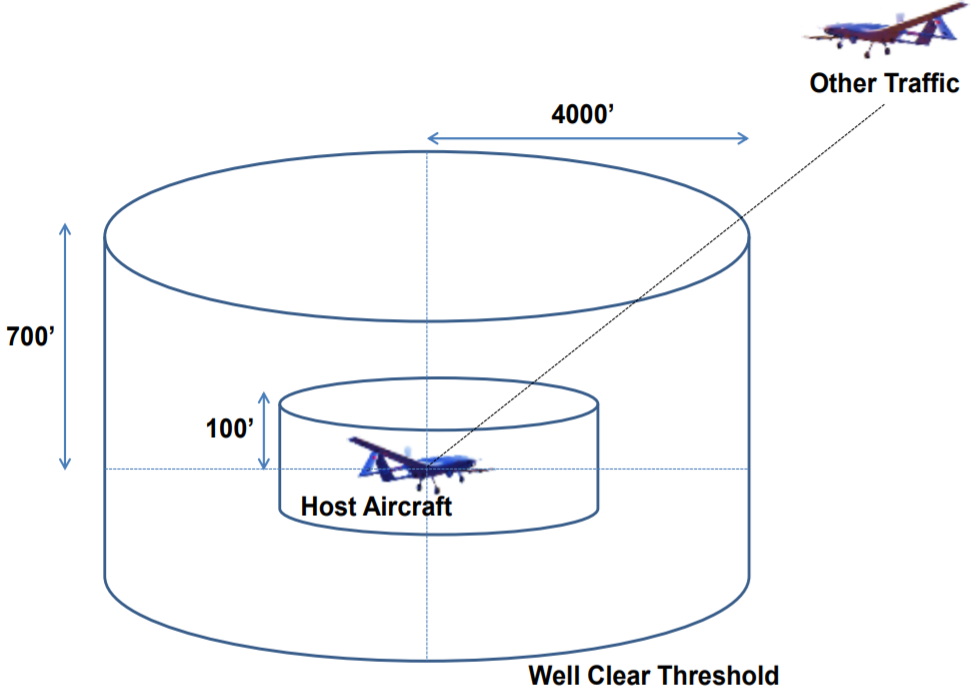
\includegraphics[width=0.6\textwidth]{\FIGDIR/02_05_WellClearTreshold}
    \caption{Well Clear Threshold \cite{valavanis2015uav,united1983pilots}.}
    \label{fig:WellClearTreshold}
\end{figure}

\noindent The boundaries and margins classification is taken from \cite{united1983pilots,valavanis2015uav} and goes like follow:

\begin{enumerate}
    \item \emph{"Alert"} - the distance to at least one surrounding aircraft is within \emph{alert margin}, the pilot is alerted about the possible threat, no action is required from pilot side.
    
    \item \emph{"Well Clear"} - the intruder enters into \emph{well clear range}, the intruder is threatening the \emph{airplane} directly, the pilot is noticed about security incident.
    
    \item \emph{"Near Miss"} - the intruder gets very close to \emph{airplane}, the body hit or \emph{turbulence impact} is very probable. 
    
    \item \emph{"Body Hit"} - the intruder stuck the \emph{airplane body}.
\end{enumerate}

\noindent These incidents are increasing their severity, the goal of separation is to keep every airspace attendant \emph{well clear}, outside well clear threshold (fig. \ref{fig:WellClearTreshold}). 
\paragraph{Air Traffic Control:} The air traffic control have passive role in separation, it manages the airspace and gives \emph{clearance} for air space users actions. There is active support for VFR (sec. \ref{sec:VisualFlightRules}) and IFR (sec. \ref{sec:InstrumentalFlightRules}). The role of \emph{Air Traffic Control} is discussed in (sec. \ref{sec:AirTrafficControl})

\paragraph{ACAS-X/TCAS:} There is support systems fo prevent \emph{Airborne Collision}, which are supporting the \emph{active avoidance} for \emph{IFR} flights (sec. \ref{sec:InstrumentalFlightRules}). Their role is to provide the surveillance of \emph{airplane} surroundings and give advisories to pilot. More about next generation system family ACAS-X can be read in (sec. \ref{sec:ACASX}). The current generation \emph{Airborne Collision} System TCAS is discussed in (sec. \ref{sec:TCAS}).


    	\subsection{(R) Air Traffic Control}\label{sec:AirTrafficControl}
\paragraph{Motivation:} The modern \emph{Air Traffic Control} (ATC) procedures are outlined in ICAO 4444 \cite{icao4444}. The ATC roles and responsibilities in terms of \emph{clearance}, \emph{self-separation}, and, \emph{provided traffic information} are summarized in (tab. \ref{tab:airspaceResponsibilitiesIcao}). 

The \emph{main role} of \emph{Air Traffic Control} (ATC) is to support the organization of the \emph{airspace} in terms of \emph{preemptive} detect and avoid.

\begin{note}
    The \emph{Reactive} and \emph{Event Based} detect and avoid for manned aviation are covered by \emph{ACAS-X/TCAS systems} (sec. \ref{sec:ACASX}, \ref{sec:TCAS})
\end{note}

\paragraph{Commands issued by ATC:} There is multiple levels of commands issued by ATC, their characteristics and compulsory level is defined as folow:

\begin{enumerate}
    \item \emph{Notification} - the information notification, commonly known as \emph{NoTice to AirMan} (NOTAM), depending on flight mode, can be transmitted as voice message or information broadcast. They usually contains information about weather and traffic situation in given sector.
    
    \item \emph{Warning} - directed message to specific general aviation  which may require some direct action. The information is usually informative, but the action is not mandatory.
    
    \item \emph{Recommendation} - directed message to specific general aviation  which requires direct action. The order is usually specific action, but the action is not mandatory to be executed by pilot.
    
    \item \emph{Directive} - directed message to specific general aviation  which requires direct action. The order is specific action and the order fulfillment is mandatory for the pilot. 
\end{enumerate}

\paragraph{Separation enforcement:} The \emph{separation} is main feature of the ATC in controlled airspace of airports (B, C, D class). Its enforced by management of \emph{action clearance}. The ATC issues the clearance for take-off/landing sequence. 

The clearance for climb/descent is given at the beginning when flight plan is approved. The ATC issues the time slots for selected pathways. The continuous monitoring of air traffic is executed in periods. The airplane deviation from cleared plan should be minimal. 

If there is any incident the the \emph{ATC} can take following actions:
\begin{enumerate}
    
    \item \emph{Heading change} - order \emph{general aviation} to change heading in given time frame (horizontal navigation). This command is usually issued to correct horizontal deviations in path tracking.
    
    \item \emph{Velocity change} - order \emph{general aviation} to change velocity in given time frame. This command is usually issued to correct time deviations in path tracking.
    
    \item \emph{Altitude change} (Flight Level) - order \emph{general aviation} to climb or descent in given time frame. This command is usually issued to correct vertical deviations in path tracking (wrong flight level).
    
    \item \emph{Divergence} - order \emph{general aviation} to follow different waypoint in flight plan (goal change). This command is usually used to resolve incidents or to reroute traffic to other hub.
    
    \item \emph{Convergence} - order \emph{general aviation} to return to following original waypoint (goal return). This command is usually used when incident have been resolved in short time and original flight \emph{path} can be re-established.
    
    \item \emph{Restrictions Enforcement} - order \emph{general aviation} to avoid some point with defined distance.  
\end{enumerate}

\begin{note}
    All ATC commands can be requested be \emph{general aviation} for clearance to be granted. Meaning the airplane can ask ATC to perform any of listed actions. 
\end{note}

The \emph{separation} can be divined into two distinctive types to form \emph{well clear barrel} (fig. \ref{fig:WellClearTreshold}). The separation types are following:

\begin{enumerate}
    \item \emph{Horizontal separation} - keep clear of any intruders on horizontal plane (flight level plane).
    
    \item \emph{Vertical separation} - keep clear of any intruders on given altitude (flight level) range.
\end{enumerate}

\begin{note}
    The \emph{horizontal/vertical} separation is enforced independently, reducing 3D avoidance problem to 2D/1D avoidance problem.
\end{note}

\paragraph{Traffic Information:} The air traffic information is delivered to general aviation depending on airspace type (tab. \ref{tab:airspaceResponsibilitiesIcao}). 

\begin{note}
    The \emph{D class} airports usually do not have a radar or transponder therefore they can provide only visual guidance in altitude/horizontal range around "control tower".
\end{note}


\paragraph{Dynamic Airspace Management:} A real-time \emph{Airspace Management} approach have been presented in \cite{gardi2014real}. Following \emph{Dynamic Airspace Management} \cite{gerdes2016dynamic}. 

The \emph{airspace is usually} divided into the \emph{clusters} where each cluster is managed by separate ATC. When airplane is leaving one cluster, airplane hand-over is executed.

There is a problem when some airspace cluster is \emph{congested} or overloaded by controlled airplanes. The example of such situation is given in (fig. \ref{fig:DAMExample}). 

\begin{figure}[H]
    \centering
    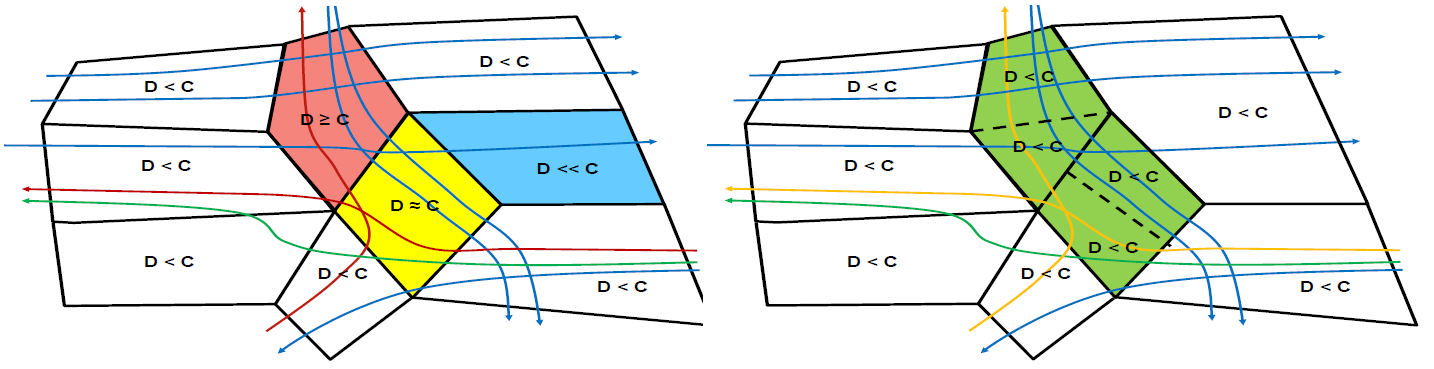
\includegraphics[width=1\textwidth]{\FIGDIR/02_02_DAM_Example}
    \caption{Example of DAM flight rerouting to homogenize traffic density \cite{gerdes2016dynamic}.}
    \label{fig:DAMExample}
\end{figure}

\begin{note}
    The air ways can not be changed, because the real time change of airways is difficult. The change of cluster authority is possible, because there is no changes for aircraft.
\end{note}

\noindent The airspace clusters are divined into three categories (fig. \ref{fig:DAMExample}):
\begin{enumerate}
    \item \emph{Under-fill} (blue) - there is less airplanes than its authority capacity.
    
    \item \emph{Saturated} (yellow) - there is enough airplanes to fill authority capacity.
    
    \item \emph{Over-fill} (red) - there is more airplanes than its authority capacity.
\end{enumerate}


\noindent The algorithm \cite{gerdes2016dynamic} will swap some airspace portions between neighbouring authorities to balance the load (all authorities should be saturated in ideal conditions) (green) (fig. \ref{fig:DAMExample}).
    	\subsection{(R) Airborne Collision Avoidance System X}\label{sec:ACASX}
\noindent This section follows the summary leaflet \cite{netalert2013n17}. The standard is still under development, the principles relevant for this work are outlined. 

\paragraph{Overview:} A development of \emph{ACAS-X} system is the FAA funded research and development program of a new approach to airborne collision avoidance. It has been ongoing since early 2008. ACAS-X approach takes an advantage of years of TCAS development. The main purpose of new system development is rapid evolution of computational capabilities and emergence of \emph{Unmanned Autonomous  Systems}.

The main purpose for manned aviation is to provide necessary advisories to pilot for \emph{Mid-Air Collision} (MAC) avoidance. There are following improvements:

\begin{enumerate}
    \item \emph{Reduce Unnecessary Advisories} - The pilot/UAS is receiving avoidance advisories or warning. 
    
    \item \emph{Extending collision avoidance to other classes of aircraft} - the current TCAS system is available mainly for bigger manned aviation, the future lies in integration of UAS systems into non-segregated airspace.
    
    \item \emph{Improvement of Surveillance Environment} - There is development in ADS-B technology and modern non cooperative sensors like LiDAR or milimeter radar, which are enhancing surviliance cappabilites of current and future airplanes.
\end{enumerate}

\paragraph{AcAS-X variants:} The \emph{ACAS-X} is not universal "\emph{one-size fits all}" system. There are multiple variations for different type of aviation:
\begin{enumerate}
    \item \emph{ACAS-X\textsubscript{P}} - the general purpose ACAS-X that makes active interrogations to establish the range of intruders. The successor to TCAS II.
    
    \item \emph{ACAS-X\textsubscript{P}} - a version of ACAS-X that relies solely on passive ADS-B to track intruders and does not make active interrogations. It is intended for general aviation (a class of aircraft not currently required to fit TCAS II).
    
    \item \emph{ACAS X\textsubscript{O}} - a mode of operation of ACAS X designed for particular operations for which ACAS-X\textsubscript{A} is unsuitable and might generate an unacceptable number of nuisance alerts (e.g. procedures with reduced separation, such as closely spaced parallel approaches).
    
    \item \emph{ACAS X\textsubscript{U}} - designed for \emph{Unmanned Aircraft Systems} (UAS).
\end{enumerate}

\begin{note}
    The \emph{ACAS X\textsubscript{U}} is mean also for \emph{reduced separation} approach in tightly packed airspace (ex. air-taxi). The determinism and \emph{false-positive} alerts occurrence minimization must be assured in order to enable UAS systems into non-segregated airspace.
\end{note}

\paragraph{ACAS-X Concept:} The \emph{ACAS-X} collision avoidance logic (fig. \ref{fig:acasxConceptScheme}) is distinguished into two phases:
\begin{itemize}
    \item[1.] \emph{Offline development phase} (Pre-calculation) similar to (sec. \ref{s:reachSet}) - ACAS-X is based on a \emph{probabilistic model} providing a statistical representation of the aircraft position in the future (position cone). It also takes into account the safety and operational objectives of the system (payload/weather/visibility/airspace/aircraft class). This enables the logic to be tailored to particular procedures or \emph{airspace configurations}.
    
    This is fed into an \emph{optimization process} called dynamic programming to determine the best course of action to follow according to the context of the conflict. This takes account of a reward (safety) to the cost (fuel consumption). The concurrent optimization enables to explore multiple maneuvers to determine which will increase \emph{separation level} (safety) and which will decrease \emph{fuel consumption} (cost).
    
    Key metrics for \emph{operational sustainability} and pilot acceptability include \emph{minimizing} the frequency of resolution advisories (UAS/GA) and traffic alerts (GA). This results into decrease of reversals/intentional intruder altitude crossing cases.
    
    \item[2.] \emph{Real-time operation} (Avoidance run) similar to (sec. \ref{s:missionControlRun}) - the \emph{look-up table} is used in real-time on-board the aircraft to resolve conflicts. An ACAS-X system collects \emph{surveillance measurements} form an array of \emph{information sources} and \emph{sensors}. The \emph{situation evaluation} is executed every second (decision time).
    
    Various models are used (e. g. a probabilistic sensor model accounting for sensor error characteristics) to estimate a state distribution, which is a probability distribution over the current positions and velocities of aircraft and intruders. The \emph{state distribution} determines where to look in the numeric look-up table to determine the best action to take. If deemed necessary \emph{Resolution Advisory} are issued to pilots/UAS control module.
    
\end{itemize}

\begin{figure}[H]
    \centering
    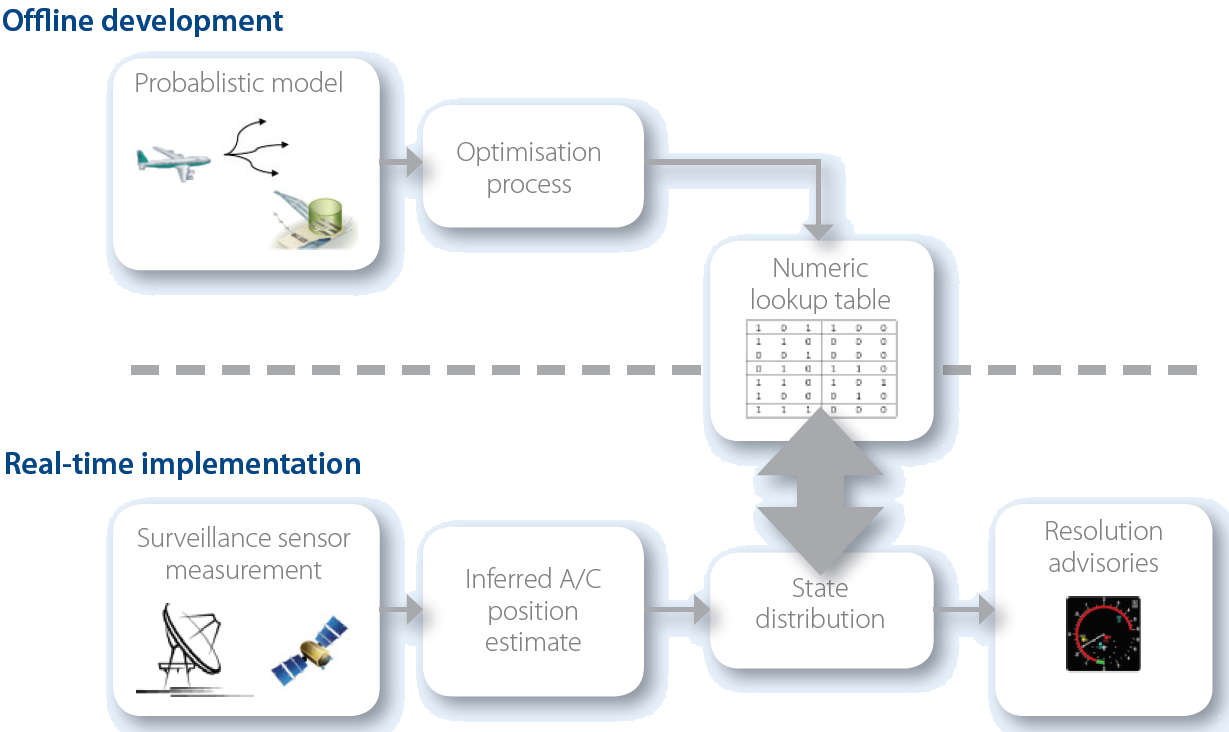
\includegraphics[width=.8\linewidth]{\FIGDIR/TE058TwoPhasesACASX}
    \caption{ACAS-X concept scheme \cite{netalert2013n17}.}
    \label{fig:acasxConceptScheme}
\end{figure}

\begin{note}
    \emph{Two-phase calculation} with offline development and real-time operation phase concept, will be used in different manner in our method. (sec. \ref{s:avoidanceConcept})
\end{note}

\paragraph{Advisories:} The \emph{ACAS-X} is taking the advisories categorization from \emph{ICAO Annex 10.} \cite{annex200710}. The advisories are recommended (directives for UAS) actions to take.


Airborne Collision Avoidance Systems (ACAS) equipment provides two types of advisories to pilots: Resolution Advisories (RAs) and Traffic Advisories (TAs). These are defined as follows:

\begin{enumerate}
    
    \item \emph{Resolution advisory} (RA) - an indication given to the flight crew recommending:
    
    \begin{enumerate}[a.]
        \item Manoeuvre intended to provide separation from all threats.
        
        \item Manoeuvre restriction intended to maintain existing separation.
    \end{enumerate}
    
    \item \emph{Corrective resolution advisory} - a resolution advisory that advises the pilot to deviate from the current flight path.
    
    \item \emph{Preventive resulution advisory} - a resolution advisory that advises the pilot to avoid certain deviations from the current flight path but does not require any change in the current flight path.

    \item \emph{Traffic advisory} (TA) - An indication given to the flight crew that a certain intruder is a potential threat.
\end{enumerate}

\begin{note}
    The \emph{UAS} system with full autonomy must handle the solution of the \emph{directives} (advisories) form UTM and other systems. The example of configurable handling mechanism - \emph{Rule engine} is given in (sec. \ref{s:RuleEngineArchitecture}).
\end{note}

\paragraph{Example Overview of the Incident:} The \emph{example of incident} and  a resolution is outlined in (fig. \ref{fig:axasxincidentoverviewexample}). The \emph{example} is given for better understanding of \emph{ACAS-X} roles \& responsibilities. 

\begin{itemize}
    \item[1.] \emph{Initial state} - the initial state is given like follow:
    
    \emph{Green Airplane} (A/C 1) is cruising on \emph{flight level} FL-390 (39 000 feet)
    
    \emph{Orange Airplane} (A/C 2) is cruising on \emph{flight level} FL-370 (37 000 feet)
    
    \item[2.] \emph{Orange aircraft transponder mishap} - the \emph{orange airplane} appears on flight level FL-405 (45 000 feet).  The \emph{green aircraft} controller (pilot) wants to \emph{descent} to oragne aircraft real flight level (FL-370). 
    
    \item[3.] \emph{Green airplane descent} - the \emph{Green aircraft} starts to descent. The \emph{Orange aircraft} keeps the flight level (FL-370). 
    
    \item[4.] \emph{Green aircraft Active Surveillance} - the \emph{green aircraft} uses \emph{active surveillance} to detect \emph{orange aircraft}. 
    
    The \emph{ACAS-X} issues \emph{Adjust Vertical Speed, Adjust - Resolution Advisory} (AVSA RA) to  the \emph{green aircraft} to \emph{level off} and stop \emph{descent} or at least slow it.
    
    Then as \emph{ACAS-X} issues \emph{Climb Resolution Advisory} to the \emph{green aircraft} mandating to get altitude. 
    
    \begin{note}
        The main issue is that \emph{pilot} is responsible decision maker, therefore pilot can refuse to follow \emph{ACAS-X advisories}.
    \end{note}
    
    \item[5.] \emph{Orange airplane starts descending} -  the \emph{orange aircraft} detects the \emph{flight level disparity} due the \emph{active surveliance} deteciton of \emph{green aircraft} on \emph{FL-370}.
    
    The \emph{Green aircraft} is tail-gating \emph{orange aircraft} from above. The \emph{ACAS-X} evaluates situation and issues a \emph{Descent Resolution Advisory} to avoid pursuit. 
    
    The \emph{pilot} of \emph{orange aircraft} follows the order of RA
\end{itemize}


\begin{figure}[H]
    \centering
    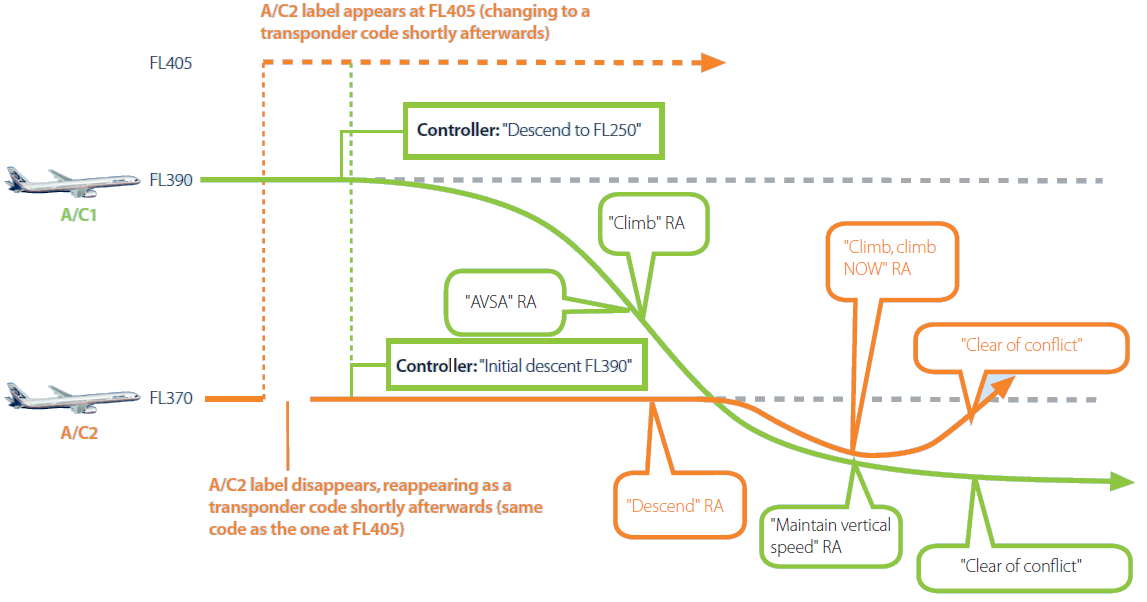
\includegraphics[width=\linewidth]{\FIGDIR/TE059ACASConflictExample}
    \caption{ACAS-X incident overview \cite{netalert2013n17}.}
    \label{fig:axasxincidentoverviewexample}
\end{figure}

\begin{itemize}
    \item[6.] \emph{Tailgating detection} - the \emph{orange airplane} is in front of \emph{green airplane}, both airplanes are descending at same rate. 
    
    \begin{note}
        This situation is very dangerous, because it is very close to \emph{intentional pursuit scenario}.
    \end{note}
    
    The \emph{orange airplane} is \emph{pursued}, its own \emph{ACAS-X} issues the \emph{Climb Now Resolution Advisory}. The pilot follows the advisory.
    
    The \emph{green airplane} is \emph{pursuing} and its goal is to \emph{descent} to flight level FL-250. Its \emph{ACAS-X} issues \emph{maintain vertical speed resolution advisory}.
    
    \item[7.] \emph{Conflict resolution} - both airplanes follow \emph{Resolution Advisories}.  When significant vertical distance is reached. The conflict is marked as resolved. 
\end{itemize}


    	\subsection{Traffic Collision Avoidance System}\label{sec:TCAS}

\noindent The \emph{TCAS} functionality is equal to ACAS-X\textsubscript{A} (sec. \ref{sec:ACASX}) functionality. The TCAS II. version 7.1 technical specification can be found in \cite{federal2011introduction}. A \emph{Resolution Advisory} (RA) detection algorithm is outlined in  \cite{munoz2013tcas}.
	
	%02-05 UTM section    
    \section{UAS Traffic Management (UTM)}\label{sec:UTM}
\paragraph{Introduction:} This section strongly follows \cite{eurocontrol2018rpasatm}, which outlined the basic concept of operations for Remotely Piloted Aerial Systems (RPAS)/Unmanned Autonomous Systems (UAS) Air Traffic Management (ATM) (later re-branded as UTM).

The \emph{RPAS/UAS} integration into \emph{non-segregated airspace} follows the general manned aviation procedure:
\begin{itemize}
    \item[$\to$] For a selected type of Operations VLOS/BVLOS/VFR/IFR:
    \begin{itemize}
        \item[$\to$] For a selected class of Air traffic (class 1. - class 7):
        \begin{itemize}
            \item[$\to$] For a selected class of airspace (class A -  class G):
            \begin{itemize}
                \item[$\to$] Deliver Operation Performance Standards ($\ge$ General Aviation)
            \end{itemize}
        \end{itemize}
    \end{itemize}
\end{itemize}

\noindent  The prototype of regulation for \emph{RPAS/UAS} standard from EASA can be found at \cite{easa2016rpasroperegul}. The section will continue with an outline of important functionality.

\paragraph{Airspace Assessment:} The future \emph{UTM} must be capable of \emph{airspace} assessment. In manned aviation, the \emph{airspace assessment} is normally triggered by either rise of traffic, environmental issues, capacity issues, and safety concerns or adapting the design to meet forecasted demands.

Presently RPAS/UAS operations have not triggered an airspace assessment s most areas are indicated as \emph{no RPAS/UAS zones}. The \emph{restricted areas} are already known on aviation maps (airport, nuclear power station, etc.). However, there are similarities with RPAS/UAS operations below 500 ft (AGL), that can trigger this requirement for an airspace assessment like, but not exclusive:

\begin{enumerate}
    \item \emph{The increase of operations density} - UAS taxi can lead to an increase in traffic density in class C and F airspaces, the UAS delivery system can lead to increased traffic density in F class airspace. 
    
    \item \emph{Introduction of BVLOS, autonomous VLOS/ELOS/BLOS operations} - current RPAS/ UAS operations are limited to VLOS which limits operation space. When this limitation is lifted, new business cases will open, leading to an \emph{increase} of RPAS/UAS traffic.
    
    \item \emph{Safety Concerns} - there is not enough accidents or critical RPAS/UAS misuse cases, to increase safety concerns, especially G class airspace does not have many manned aviation parallels.
    
    \item \emph{Environmental Aspect} - the RPAS/UAS is not constructed from clean and safe materials, any accident can lead to serious habitat damage (ex. gasoline in water reservoir).
\end{enumerate}

The \emph{assessment} should develop a new type of airspace organization able to cater to the new demand of operations and ensure safety levels are met. The airspace assessment can take into considerations the following aspects:

\begin{enumerate}
    \item \emph{Airspace classification} - further airspace decomposition in F/G  uncontrolled airspace to establish \emph{flight routes} and controlled areas. Further flight levels in C class airspace segmentation to enforce manned/unmanned aviation separation.
    
    \item \emph{Traffic complexity and density} - the \emph{congestion} of traffic is very common on the road. The capability to stop or stay still in the air is very costly to implement and maintain both in manned/unmanned aviation.
    
    \item \emph{Geographical situation} - flat-lands vs. mountains, urban vs. rural areas.
    
    \item \emph{Privacy} - in \emph{very low altitude} operations the privacy is always a concern.  The current restrictions to flew over private properties needs to be lifted in order to enable increased higher traffic density.
    
    \item \emph{Security} - the \emph{UTM} and \emph{RPAS/UAS} systems are creating a network of \emph{autonomous agents}; this network is venerable to any kind of \emph{cyber/physical} threat.
\end{enumerate}

\paragraph{Types of RPAS/UAS operations:} The \emph{future UTM functionality} must cover a wide range of functionality. It is envisaged that RPAS/UAS will operate in a mixed environment adhering to the requirements of the specified airspace it is operating in. RPAS/UAS will be able to operate as follows:

\begin{enumerate}
    \item \emph{Very Low-Level (VLL) operations} ($<500 feet (AGL)$).
    
    \item  \emph{IFR (Instrumental Flight Rules) or VFR (Visual Flight Rules)} ($500 feet \le altitude < 60 000 feet (AMSL)$) - following the same rules that apply to manned aircraft. These can be conducted in RLOS or B-RLOS conditions.
    
    \item  \emph{Very High-Level operations (VHL suborbital IFR operations above FL600)} ($\ge$ $60 000$ $feet$ $(AMSL)$).
\end{enumerate}

\paragraph{VLL operations (Below 500 feet AGL):} Operations performed at altitudes below 500 feet are not new to manned aviation as many operators - police, armed forces, balloons, gliders, training crafts, fire-fighting, ultra-light aircraft are allowed to operate in this environment. The rule allows VFR traffic to operate, under specific conditions prescribed by the competent national authorities, conditions that can differ from State to State. RPAS/UAS operating in this volume of airspace do not however confirm either IFR or VFR as given in ICAO Annex 2. \cite{icaoAnnex2}.

\begin{enumerate}
    \item \emph{VLOS (Visual Line Of Sight)} - RPAS/UAS operations within 500 meters range and max 500 feet  altitude from the a pilot. One of the main responsibilities of the pilot is the safe execution of the flight through visual means. The distance can be increased by the use of one or more observers, sometimes referred to as Extended-VLOS (E-VLOS).
    
    \item \emph{BVLOS (Beyond Visual Line Of Sight)} -  RPAS/UAS operations beyond 500 meters range but below 500ft. BVLOS does not require the operator to ensure the safety of the flight visually, and technical solutions such as DAA and C2 data link are required. RPAS/UTM does not adhere to VFR or IFR requirements; however, it is foreseen that these flights could be conducted in IMC or VMC conditions. BVLOS operations are already being conducted in several States. Some examples are:
    
    \begin{enumerate}[a.]
        \item Power-line control.
        
        \item Maritime surveillance.
        
        \item Pipeline control.
        
        \item  Agriculture.
    \end{enumerate}
\end{enumerate}

\noindent\emph{VLL Management System:} In order to accommodate the expected growth of traffic in this airspace and ensure a sufficient level of safety, it is anticipated the necessity for a supporting UTM system. This VLL Traffic Management system will provide a series of localization and information services, aiming to the provision of information to the RPAS pilots and manned traffic. The VLL UTM system will not provide an active control service for RPAS in a normal ATC fashion, due to a large number of RPAS/UAS involved. Such a system could be based on existing technologies, such as the mobile phone network. Specific RPAS/UAS reporting systems, providing authorization and information capability, are already in use in several states.

The RPAS/UAS management system will have to cater to the following aspects:

\begin{enumerate}
    \item  RPAS/UAS Flight planning.
    
    \item  RPAS/UAS Flight authorization.
    
    \item  Real-time RPAS/UAS tracking capability.
    
    \item  Provision of actual weather and aeronautical information.
\end{enumerate}

\noindent As previously mentioned, it is envisaged that the VLL management system will not support the active controlling of RPAS/UAS at lower altitudes. The large number of RPAS/UAS will not make this possible, notwithstanding any liability aspects. The system will be supporting operations and will be able to provide sufficient data to safely execute an RPAS/UAS flight, based on the information available to it. Data required could include, but are not limited to:

\begin{enumerate}
    \item Planned flight plans.

    \item Active RPAS/UAS flight plans/missions.

    \item Airspace data.

    \item NOTAM (NOtice To AirMan).
    
    \item Weather.

    %\item Infrastructure availability.

    \item Geo-fencing.

    \item Manned operations below 500 feet (AGL).
\end{enumerate}



\noindent The following assumptions have been made for future ATM/UTM systems:
\begin{enumerate}
    \item A C2 service is provided.

    \item The State has executed airspace, and assessment geo-fencing is in place.
    
    \item  RPAS/UAS have surveillance capability similar concerning performance and compatible to manned aircraft surveillance capability.
    
    \item  Specific RPAS/UAS traffic management system is in place.
\end{enumerate}

\begin{note}
    RPAS/UTM vehicle categorization is outlined in \emph{U-SPACE section} (sec. \ref{sec:USpace}).
\end{note}

\noindent The classification of traffic in this airspace segment goes like follow:


\paragraph{Class I.:} Class I traffic is primarily reserved for RPAS Category A (buy and fly). In areas of low traffic density this class can operate from the ground up to 500ft and is a subject to the following requirements:
    \begin{itemize}
        \item[1.]  Mandatory declaration of operation.
        
        \item[2.]  RPAS must be capable to self-separate in 3D.
        
        \item[3.]  VLOS operations only.
        
        \item[4.]  Geo-fencing capability which ensures that this category remains separated from no-drone zones.
    \end{itemize}
    
\paragraph{Class II.:} Class II traffic operates in free flight due to the nature of their operations like Surveys, filming, search and rescue and other operations that have no fixed route structure. Class II can operate from the ground up to 500 feet (AGL) and is a subject to the following requirements:
    \begin{itemize}
        \item[1.] Mandatory authorization for operation.
        
        \item[2.] Surveillance capability (C2 4G chip or other means).
        
        \item[3.] VLOS and BVLOS operations.
        
        \item[4.]  Free flight Capability.
        
        \item[5.]  RPAS/UAS must be capable to self-separate in 3D.
        
        \item[6.]  BVLOS will have barometric measurement equipage.
    \end{itemize}
    
    
\paragraph{Class III.:} Class III traffic only operates in BVLOS and is mainly used for transport purposes. It can operate as free flight or within a route structure pending on the requirements set by the airspace assessment.
    \begin{itemize}
        \item[1.] Mandatory authorization for operation.
        
        \item[2.] Has surveillance capability.
        
        \item[3.] BVLOS operations only.
        
        \item[4.] Free flight or route structure.
        
        \item[5.] Shall have barometric measurement equipage.
        
        \item[6.] Can operate from the ground up to 500 ft.
    \end{itemize}
    
\paragraph{Class IV.:} Class IV traffic can operate within the layer between the ground and 500 feet. This category is designed for highly specialized operations and as such not many of these types RPAS/UAS are expected. These can be civil, state or military operations and as such:
    \begin{itemize}
        \item[1.] Require special authorization.
        
        \item[2.] Should be addressed on a case by case basis.
        
        \item[3.] VLOS and BVLOS.
        
        \item[4.] Could require surveillance capability.
    \end{itemize}

\paragraph{IFR/VFR Operations (between 500ft - FL 600):} For RPAS/UAS to fly either IFR/VFR requires that they meet the airspace requirements as set for manned aviation. These operations include airports, TMA and Enroute. For IFR capable RPAS additional requirements can be set for flying in the volumes of airspace where normal transport aircraft operate. As such it is envisaged to have minimum performance standards for elements such as speed, climb/descent speed, turn performance and latency.

\emph{Operations of Small RPAS above 500 feet:} In principle operations above 500 feet by small RPAS/UAS are not allowed unless they meet the IFR/VFR airspace requirements and have a solution to be visible to manned traffic. Other aspects like wake turbulence and separation standards would also have to be addressed. However, States can still on a case by case basis accommodate RPAS/UAS above 500ft if the risk assessment of the intended operation is acceptably low.

\noindent The classification of traffic in this airspace segment goes like follow:

\paragraph{Class V.:} Class V is IFR/VFR operations outside the Network not flying SIDs and STARs. In this environment, RPAS/UAS not meeting Network performance requirements will be able to operate without negatively impacting manned aviation. Operations at airports will be accommodated through segregation of launch and recovery.

    Ground operations can also be accommodated through either towing or wing walking.

    Operations from uncontrolled airports or dedicated launch and recovery sites are to be conducted initially under VLOS/VFR until establishing radio contact with ATC.

    No additional performance requirements will be set in this environment compared to manned aviation.
    
    RPAS/UAS operating in the environment will file a flight plan including information such as:
    \begin{itemize}
        \item[1.] Type of RPAS/UAS, 2. Mission plan, 3. Contingency procedure.
        
        \item[4.] RPAS/UAS will meet CNS airspace requirements.
        
        \item[5.] RPAS/UAS will be able to establish two-way communication with ATC/UTM if required.
        
        \item[6.]  RPAS/UTM will remain clear of manned aircraft.
        
        \item[7.]  RPAS operator must be able to contact ATC/UTM (if required) regarding special conditions such as data link loss, emergency, controlled termination of flight.
        
        \item[8.] RPA/UTM DAA capability will be cooperative with existing ACAS systems.
    \end{itemize}
    
\paragraph{Class VI.:} Class VI. is IFR operations, including Network, TMA and Airport operations with RPAS/UAS capable of flying SIDs and STARs as designed for manned operations. These are either manned transport aircraft enabled to fly unmanned with similar capabilities or new types able to meet the set performance requirements for the Network, TMA and airports. General requirements RPAS/UAS operating in this environment will file a flight plan (mission) including:
    \begin{itemize}
        \item[1.] Type of RPAS/UAS.
        \item[2.] Contingency procedure.
        \item[3.] Mission plan (navigation, route, level).
        \item[4.] RPAS/UAS will meet CNS airspace requirements.
        \item[5.] RPAS/UAS will be able to establish two-way communication with ATC/UTM.
        \item[6.] RPAS/UAS operator must be able to contact ATC (if required) in regard regarding special conditions such as data link loss, emergency, controlled termination of flight.
        \item[7.] RPAS/UAS DAA capability will have ACAS functionality.
    \end{itemize}

\begin{note}
    The class operation class $V.-VI.$ is covered mostly in this work.
\end{note}

\paragraph{VHL operations (Above FL 600):} Suborbital unmanned flights operating at altitudes above FL 600 are expected to grow fast in numbers. Apart from military HALE RPAS, several other vehicles (i.e., space rockets, Virgin Galactic, etc.) operate through or in this block of airspace. At this moment, no management of this traffic is foreseen in most parts of the world. Particular attention should be given to the entry and exit of this high altitude volume as they need to interact with the airspace below.

\noindent The classification of traffic in this airspace segment goes like follow:


\paragraph{Class VII.:} Class VII consists solely of IFR operations above FL600 and transiting non-segregated airspace.
    
    These types of RPAS/UAS are solely designed for operations at very high altitudes. The launch and recovery of fixed-wing RPAS/UAS can be from dedicated airports and outside congested airspace unless Class VI requirements are met. This airspace will be shared with many different RPAS/UAS. Although their operations will not directly impact the lower airspace, however, they will have to transit through either segregated or non-segregated airspace to enter or exit the airspace above FL 600.
    
    For such cases, temporary segregated airspace should be considered. Transition performance in segregated or non-segregated airspace below FL600 will be very limited since they will be focusing on long missions (up to several months).

    The airspace in which these types of operation take place is mostly seen as uncontrolled. This requires no management of this traffic; however due to the expected numbers - estimated to be around 18000 just for Google and Facebook - it will become necessary to manage this type of operation since the performance envelopes differ a lot. Speeds can vary from average wind speed at those altitudes (for Google balloons) up to above-mach.

    Launch and recovery of unmanned balloons or aircraft, together with emergency situations, will also require a set of procedures and pre-arranged coordination capabilities to ensure the safety of traffic below this altitude.



    	\subsection{U-Space}\label{sec:USpace}

\noindent The \emph{Concept Of OpeRations of U-Space} (CORUS) \cite{corus2018} has been released recently. This concept describes the difference between the standard ATM and proposed European UTM solution. This section will get through the interesting part of this pivotal document.

\newpage\noindent The \emph{U-space} is separated into following functionality based phases:
\begin{itemize}
    \item[\texttt{U1}] (year $<$ 2020) - sets the scene with registration and geo-fencing.
    
    \item[\texttt{U2}] (year$<$ 2025) - introduces tracking, flight planning and messages sent to the remote pilot during flight.
    
    \item[\texttt{U3}] (year$<$ 2030) introduces collaborative detect and avoid and tactical conflict resolution.
    
    \item[\texttt{U4}] (year $<$ 2035) brings safe interoperation with manned aviation.
\end{itemize}

The \emph{Aspects} important for \emph{Obstacle avoidance} will be outlined and discussed over this section. Our work focuses on \emph{European Airspace} (EASA); therefore more focus will be on \emph{U-space}

\paragraph{Small UAS Classification:} Manned aviation is covered by existing rules, for example \cite{icaoAnnex2,ec201208ref5}. Excluding some specific situations, manned aviation does not fly below VFR airspace, do not enter \emph{very low level} (VLL) altitudes \cite{ec200802ref4}. 

The certified airworthiness is mandatory for \emph{airspace attendants} with \emph{Maximum Take-Off Mass} (MTOM) over $150 kg$. The other \emph{airspace attendants} need to fulfill only \emph{Minimal Operation Performance Specification} (MOPS). 

In \cite{easa201801op} EASA proposed several classes for UAS below $150kg$ MTOM; see Appendix 1 of the annex to Opinion 1-2018 entitled "…on making available on the market of unmanned aircraft intended for use in the ‘open’ category" and on third-country UAS operators. In that text, the next smaller mass mentioned below 150kg is 25kg MTOM. A similar break is proposed in some national legislation, for example in the UK at 20kg. As a working definition, this little chart shows a possible breakdown by MTOM. Note
that EASA classes depend on many factors, not only MTOM.

\begin{table}[H]
    \centering
    \begin{tabular}{c||c|l}
    \begin{tabular}[c]{@{}c@{}}EASA\\ class\end{tabular} & \begin{tabular}[c]{@{}c@{}}Maximum \\ take-off mass\end{tabular} & Remarks \\\hline\hline
     C0 & $\le 250 g$   & "Child`s Toy" with very limited capabilities \\\hline
     C1 & $\le 900 g$   & "Adult`s Toy" small flying camera \\\hline
     C2 & $\le 4 kg$    & "Small UAS" with the package \\\hline
     C3 & $\le 25 kg$   & "Standard UAS" attainable AGL altitude $\le 120m$ \\\hline
     C4 & $\le 25 kg$   & "Standard UAS" no automatic control mode  altitude $> 120m$\\\hline
     -  & $\le 150 kg$  & "Heavy UAS", not defined in \cite{easa201801op} \\\hline
     -  & $> 150 kg kg$ & Regulated by EASA like the manned aircraft \cite{ec200802ref4} 
    \end{tabular}
    \caption{Small UAS Classes according to EASA. \cite{corus2018}}
    \label{tab:smallDroneClessesAccordingtoEASA}
\end{table}

\begin{note}
    The class C3 and C4 are different in operational restrictions. This work focuses mainly on UAS classes C2/C3/C4 because they have enabled \emph{automatic control mode} 
\end{note}
\newpage
\paragraph{Separation Minima:} The \emph{Separation Minima} defines \emph{minimal distances} between airspace attendants to ensure secure \emph{operation}.  The separation minima are taken from Corus \cite{corus2018}. 

All ideas for safe concurrent operation of UAS are based on the idea of keeping the UAS systems apart or physically distant from some risk source. 

A geo-fence, for example, is simply a method of providing separation. There will need to be separation minima for UAS just as there are for manned aircraft and these will be needed by services such as Monitoring which seeks to warn about loss of separation and Tactical Conflict Resolution which may act to avoid the loss of separation.

Separation minima will be different from those for manned aircraft as small UAS systems are generally much smaller and often slower moving than manned aircraft. CORUS proposes the following as separation minima (tab. \ref{tab:proposedseparationMinimaforUAS})

\begin{table}[H]
    \centering
    \begin{tabular}{l||l|l|l}
        \multicolumn{1}{c||}{\begin{tabular}[c]{@{}c@{}}Flight Type\\ Interaction\end{tabular}} & \multicolumn{1}{c|}{Horizontal} & \multicolumn{1}{c|}{Vertical|} & \multicolumn{1}{c}{Remark} \\\hline\hline
        %TableLine 1
        \begin{tabular}[c]{@{}l@{}}
            Any UAS - Manned or\\
            person carrying
        \end{tabular} & 
        \begin{tabular}[c]{@{}l@{}}
            2.5 NM
        \end{tabular} & 
        \begin{tabular}[c]{@{}l@{}}
            500 ft
        \end{tabular} & 
        \begin{tabular}[c]{@{}l@{}}
            Half the current manned\\
            aircraft separation
        \end{tabular}\\\hline
        
        %TableLine 2
        \begin{tabular}[c]{@{}l@{}}
            VLOS - VLOS
        \end{tabular} & 
        \begin{tabular}[c]{@{}l@{}}
            Remain\\
            "Well Clear"
        \end{tabular} & 
        \begin{tabular}[c]{@{}l@{}}
            Remain\\
            "Well Clear"
        \end{tabular} & 
        \begin{tabular}[c]{@{}l@{}}
            The remote pilot is not\\
            expected to judge distance by\\
            sight from the remote piloting\\
            position.
        \end{tabular}\\\hline
        
        %TableLine 3
        \begin{tabular}[c]{@{}l@{}}
            VLOS - BVLOS
        \end{tabular} & 
        \begin{tabular}[c]{@{}l@{}}
            Remain\\
            "Well Clear"\\
            + 200 ft
        \end{tabular} & 
        \begin{tabular}[c]{@{}l@{}}
            Remain\\
            "Well Clear"\\
            + 200 ft
        \end{tabular} & 
        \begin{tabular}[c]{@{}l@{}}
            The remote pilot is not\\
            expected to judge distance by\\
            sight from the remote piloting\\
            position.
        \end{tabular}\\\hline
        %TableLine
        \begin{tabular}[c]{@{}l@{}}
            BVLOS – BVLOS
        \end{tabular} & 
        \begin{tabular}[c]{@{}l@{}}
            200 ft
        \end{tabular} & 
        \begin{tabular}[c]{@{}l@{}}
            150 ft
        \end{tabular} & 
        \begin{tabular}[c]{@{}l@{}}
            Figures come from a \\
            pessimistic estimate of\\
            satellite navigation\\
            performance.
        \end{tabular}
\end{tabular}
    \caption{Proposed separation minima for UAS. \cite{corus2018}}
    \label{tab:proposedseparationMinimaforUAS}
\end{table}

\begin{note}
    The \emph{BVLOS – BVLOS} separation minima are interesting because the \emph{autonomous mode} is considered as BVLOS to  BVLOS avoidance in case of autonomous UAS.
    
    The \emph{separation minima} for \emph{UAS - Manned aviation} is unreasonably huge (2 nautical miles), and in current it should be considered as moving constraint.
\end{note}

\newpage
\paragraph{Flight Rules:} The \emph{aspects} of UAS flight rules for U-SPACE concept is summarized in the table:
\begin{table}[H]
    \centering
    \begin{tabular}{l||l}
        \multicolumn{1}{c||}{
        \begin{tabular}[c]{@{}c@{}}
            Aspect
        \end{tabular}} & 
        %\multicolumn{1}{c}{Hobby Flight Rules} &
        \multicolumn{1}{c}{UAS Flight Rules} \\\hline\hline
        %riadok 1
        \begin{tabular}[c]{@{}l@{}}
            Flight plan required
        \end{tabular} & 
        %\begin{tabular}[c]{@{}l@{}}
        %    No, but allowed
        %\end{tabular} & 
        \begin{tabular}[c]{@{}l@{}}
            Yes
        \end{tabular}\\\hline
        %riadok 2
        \begin{tabular}[c]{@{}l@{}}
            Allowed flight type
        \end{tabular} & 
        %\begin{tabular}[c]{@{}l@{}}
        %    VLOS, EVLOS
        %\end{tabular} & 
        \begin{tabular}[c]{@{}l@{}}
            VLOS, EVLOS, BVLOS
        \end{tabular}\\\hline
        %riadok 3
        \begin{tabular}[c]{@{}l@{}}
            Provision of separation in U1,\\
            VLOS \& EVLOS
        \end{tabular} & 
        %\begin{tabular}[c]{@{}l@{}}
        %    Pilot
        %\end{tabular} & 
        \begin{tabular}[c]{@{}l@{}}
            Pilot
        \end{tabular}\\\hline
        %riadok 4
        \begin{tabular}[c]{@{}l@{}}
            Provision of separation in U1,\\
            BVLOS
        \end{tabular} & 
        %\begin{tabular}[c]{@{}l@{}}
        %    N/A
        %\end{tabular} & 
        \begin{tabular}[c]{@{}l@{}}
            Geo-fence / Geo-cage
        \end{tabular}\\\hline
        %riadok 5
        \begin{tabular}[c]{@{}l@{}}
            Provision of separation in U2
        \end{tabular} & 
        %\begin{tabular}[c]{@{}r@{}l@{}}
        %    1. & Pilot (visual)\\
        %    2. & Limited support may be\\
        %       & obtained by using a Traffic\\
        %       & Information Service\\
        %\end{tabular} & 
        \begin{tabular}[c]{@{}r@{}l@{}}
            1. &  Strategic Conflict Resolution\\
               &  enabled by flight planning\\
            2. &  Traffic Information Service\\
               &  enabled by position reporting\\
            3. &  Pilot (visual)\\
        \end{tabular}\\\hline
        %riadok 6
        \begin{tabular}[c]{@{}l@{}}
            Provision of separation in U3 \&\\
            U4
        \end{tabular} & 
        \begin{tabular}[c]{@{}r@{}l@{}}
            1. &   Strategic Conflict Resolution\\
               &   enabled by flight planning\\
            2. &   Traffic Information Service\\
               &   enabled by position reporting\\
            3. &   Cooperative Tactical\\
               &   Conflict Resolution\\
            4. &   Detect and Avoid\\
            5. &   Pilot (visual)
        \end{tabular}\\\hline
        %riadok 7
        \begin{tabular}[c]{@{}l@{}}
            Separation from manned\\
            aviation in U2, VLOS or EVLOS\\
            UAS flight
        \end{tabular} & 
        \begin{tabular}[c]{@{}l@{}}
            The pilot is responsible\\
            to get the UAS out of the way\\
            of the manned aircraft.\\
        \end{tabular}\\\hline
        %riadok 8
        \begin{tabular}[c]{@{}l@{}}
            Separation from manned\\
            aviation in U2, BVLOS UAS\\
            flight\\
        \end{tabular} & 
        \begin{tabular}[c]{@{}l@{}}
            Flight plan required from both.\\
            Separation by planning.\\
            BVLOS pilot should use traffic\\
            information to avoid the\\
            manned aircraft (which is\\
            tracked).
        \end{tabular}\\
    \end{tabular}
    \caption{Aspects of UAS flight rules.\cite{corus2018}}
    \label{tab:aspectsOfUasFlightRules}
\end{table}

\noindent Following \emph{detect and avoid} requirements can be outlined based on (tab. \ref{tab:aspectsOfUasFlightRules}).
\begin{enumerate}
    \item \emph{Separation in U1} - only \emph{identification services} are provided in this phase. The \emph{Detect And Avoid} support can be provided only to UAS pilot in the form of visual or sound advisories. 
    
    \item \emph{Separation in U2} - the \emph{position notifications} are added, enabling, preemptive collision avoidance by flight planning (mission control). The \emph{traffic information} can be added to pilot software for better situation awareness.  


    \item \emph{Separation in U3 \& U4} - the \emph{advanced} avoidance concepts, from our perspective following aspects are interesting: 
    \begin{enumerate}[a]
        \item \emph{Cooperative Tactical Conflict Resolution} - The UTM infrastructure and hierarchy for \emph{cooperative conflict} resolution must be established. In form of UTM \emph{directives} and UAS \emph{fulfillment}.
        
        \item \emph{Detect and Avoid} - reactive obstacle/intruder avoidance and situation awareness on a very high level.
    \end{enumerate}
    
    \item \emph{Separation from Manned Aviation} - the \emph{well clear threshold} (fig. \ref{fig:WellClearTreshold}) for manned aviation  (tab.\ref{tab:proposedseparationMinimaforUAS}) are too big. The \emph{effective} application of \emph{reactive obstacle avoidance} is not reasonable, because the manned aviation will be out of range for most sensors (except ADS-B).
\end{enumerate}

\begin{note}
    Our work covers \emph{cooperative conflict resolution} and \emph{detect \& avoid}.
\end{note}

\paragraph{Geo-fencing Modes:} A Geo-fencing appears in U1, U2, and U3 and is successively refined. It is supported by aeronautical information for UAS systems. This table summarizes the different features by level:

\begin{table}[H]
    \centering
    \begin{tabular}{l||l|l}
        \multicolumn{1}{c||}{Capability} & \multicolumn{1}{c|}{Level} & \multicolumn{1}{c}{Features} \\\hline\hline
        %line 1
        \begin{tabular}[c]{@{}l@{}}
            Pre-Tactical \\Geo-Fencing
        \end{tabular} & 
        \begin{tabular}[c]{@{}l@{}}
            U1
        \end{tabular} & 
        \begin{tabular}[c]{@{}l@{}}
            Information provided before flight. The user should have\\
            access to AIP and NOTAM defined geo-fences in a form that\\
            can be used when planning and that can be loaded onto the\\
            UAS if it has geo-fence fence features in its navigation\\
            system
        \end{tabular}\\\hline
        %line 2
        \begin{tabular}[c]{@{}l@{}}
            On-board \\Geo-Fencing
        \end{tabular} & 
        \begin{tabular}[c]{@{}l@{}}
            U1
        \end{tabular} & 
        \begin{tabular}[c]{@{}l@{}}
            The ability of the UAS to keep itself on the correct side of a\\
            geo-fence by having geo-fence definitions (location, time,\\
            height) within its navigation system\\
        \end{tabular}\\\hline
        %line
        \begin{tabular}[c]{@{}l@{}}
            Tactical \\Geo-Fencing
        \end{tabular} & 
        \begin{tabular}[c]{@{}l@{}}
            U2
        \end{tabular} & 
        \begin{tabular}[c]{@{}l@{}}
            This service delivers to the pilot and /or UAS operator\\
            updates to and new definitions of Geo-Fences occurring at\\
            any time, including during flight.\\
            The creation of geo-fences with immediate effect require\\
            that they are defined outside the AIP. 
        \end{tabular}\\\hline
        %line
        \begin{tabular}[c]{@{}l@{}}
            UAS \\Aeronautical\\
            Information\\ Management
        \end{tabular} & 
        \begin{tabular}[c]{@{}l@{}}
            U2
        \end{tabular} & 
        \begin{tabular}[c]{@{}l@{}}
            U2 include a non-AIP repository of Geo-Fences. The\\
            UAS Aeronautical Information Management service\\
            includes all information coming from such a source,\\
            combined with information from the AIP and NOTAMS\\
            together with any other UAS relevant sources.
        \end{tabular}\\\hline
        %line
        \begin{tabular}[c]{@{}l@{}}
            Dynamic\\Geo-Fencing
        \end{tabular} & 
        \begin{tabular}[c]{@{}l@{}}
            U3
        \end{tabular} & 
        \begin{tabular}[c]{@{}l@{}}
            This service delivers updates definitions of geo-fences\\
            directly into the UAS, even in flight. This service\\
            relies on capabilities of the UAS in U3 to receive\\
            communications from U-space and to deal with geo-fence\\
            updates.
        \end{tabular}
    \end{tabular}
    \caption{Geo-fencing in U-space. \cite{corus2018}}
    \label{tab:geofencingInUspace}
\end{table}

\noindent The \emph{impact of geo-fencing} on \emph{Detect and Avoid} system is following:
\begin{enumerate}
    \item \emph{Pre tactical} - The \emph{flight plan} (mission) is prepared to avoid all \emph{known forbidden areas}. In this phase, the geo-fence covers static space constraints.
    
    \item \emph{Onboard} - The \emph{flight plan} (mission) specification does not contain all static space constraints. These constraints are known prior the flight. If UAS approaches such constraints, it needs to avoid them. The concept of soft constraints - restricted, but breakable space constraints emerge. 
    
    \item \emph{Tactical} - The \emph{space constraints} are updated during the flight. This can also be used for notifying the weather situations, restricted airspace, and all sort of \emph{static or moving constraints}.
    
    \item \emph{Dynamic} - The \emph{space constraints} the updates are real time.
\end{enumerate}

\begin{note}
    The work covers dynamic and tactical \emph{Geo-fencing}.
\end{note}

\paragraph{Actively maintaining separation during flight:} The standard ATM functionality \cite{icao4444} and \emph{Rules Of the Air} \cite{icaoAnnex2,icaoAnnex11} are covered and to be implemented for \emph{U-Space}.
    	\subsection{\secState{R}NASA UTM}\label{sec:NASAUtm}

\noindent The \emph{NASA UTM}\footnote{Related research and articles: \url{https://utm.arc.nasa.gov/documents.shtml}} is UAS Traffic Concept developed by \emph{National Aeronautics and Space Administration} (NASA) in cooperation \emph{Federal Aviation Administration} (FAA). The \emph{concept} is very similar to \emph{EASA U-SPACE}.

\begin{note}
    This work is focused on \emph{European Airspace}; the \emph{details} will be omitted. 
\end{note}

\paragraph{Useful concepts:} The \emph{NASA UTM} concept has greater maturity level concerning \emph{Detect \& Avoid} concept than European \emph{U-Space}. There is vast amount of publications which can be used in \emph{U-Space} from these publications the following useful studies containing DAA concepts were taken into account:

\begin{enumerate}    
    \item The non-cooperative intruder avoidance concept \cite{cone2017uas} provides a general idea about the \emph{topic}. The \emph{vertical separation} and \emph{vertical encounter model} is presented.
    
    \item The \emph{Detect and Avoid} performance evaluation is crucial for system performance assessment. The assessment framework \cite{lee2016wide} provides us with methodological guidelines. The used concepts are abstracting the multidimensional performance criteria into simple metrics:
    
    \begin{enumerate}[a.]
        \item \emph{Crash Distance} - the distance to the obstacle/intruder margin.
        
        \item \emph{Safety Margin} - the virtual margin around obstacle/intruder.
    \end{enumerate}
    
    \item To \emph{Ensure} the compatibility between \emph{UAS Detect And Avoid System} and \emph{Manned Aviation Collision Avoidance} (ACAS/TCAS) systems the following approach was proposed \cite{thipphavong2017ensuring}.
\end{enumerate}

    	
    %02-06 Event Based Avoidance
    \section{(W) Event Based Avoidance}\label{sec:EventBasedAvoidance}
\begin{itemize}
    \item Introduce the context for Event based avoidance: 
    \begin{itemize}
        \item Preventive DAA - before flight preparation
        \item Event-based DAA - reaction window in minutes, usually cooperative via notifications and other methods
        \item Reactive DAA - you know the drill boys ..., reaction window in 10th of seconds ...
    \end{itemize}
    \item Introduce the process of notification and Event Resolution
    \item Outline hierarchy in U(A)TM controlled space 
    \item Outline expected minimal set of data sources
\end{itemize}

\subsection{(W) Mid-Air Collision Prevention}\label{sec:MidairCollisionPrevention}
\begin{itemize}
    \item Identify and dispute shortcomings of Aircraft classification in ICAO
    \item List of MAC events
    \item For each event describe trigger and resolution 
    \item cite barrel \cite{welzl1991smallest}
\end{itemize}

\subsection{(W) Weather Impact}\label{sec:WeatherImpact}

    \begin{itemize}
        \item do not use term "climate change"
        \item critical events are getting more localized and their magnitude is increased
        \item List of Weather event
        \item Discuss weather mitigation
    \end{itemize}
    
    \emph{Weather Impact} on transportation in general has been introduced by Koetse in study \cite{koetse2009impact}.
    
    \emph{Weather-based} preemptive planning have been introduced into manned aviation in 2015 \cite{yamashita2015climate}. \TBD{This one shows global model impact}
    
    \emph{Severe Weather Condition Detection Capabilities} for current level of standard aviation equipment have been reviewed in \cite{smith2016multi} \TBD{This one shows intermediate weather detection}
    
    \begin{figure}[H]
	\centering
	\begin{subfigure}{0.45\textwidth}
		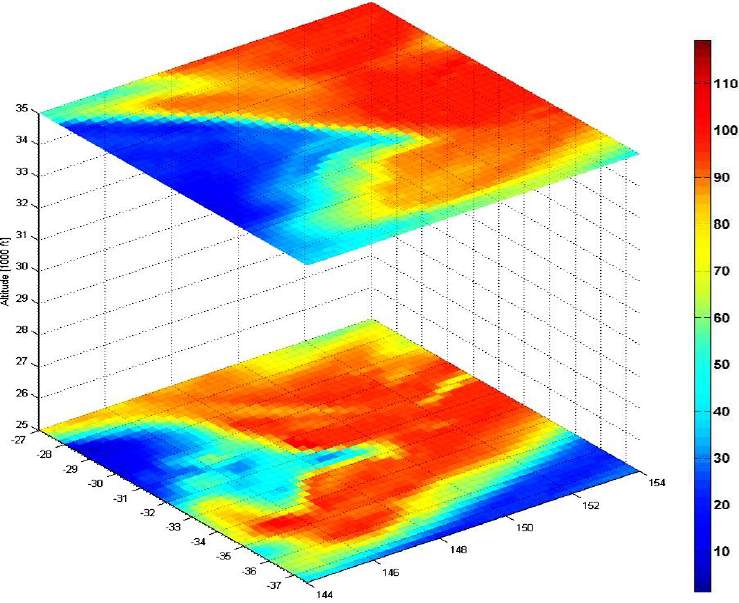
\includegraphics[width=\textwidth]{\FIGDIR/02_03_RelativeHumidity}
		\caption{Relative Humidity.} 
	\end{subfigure}
	\vspace{1em} 
	\begin{subfigure}{0.45\textwidth} % width of right subfigure
		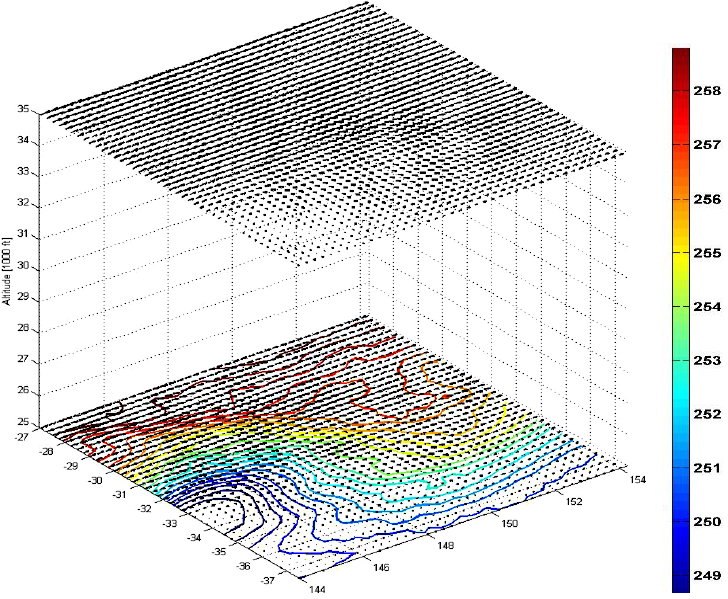
\includegraphics[width=\textwidth]{\FIGDIR/02_04_WindTemperature}
		\caption{Localized Wind Vectors.} % subcaption
	\end{subfigure}
	\caption{Localized Weather Model \cite{balaban2017dynamic}.} % caption for whole figure
    \end{figure}
    
    \emph{Icing risk} in localized environment have been predicted based on numerical model \cite{thompson2017numerical}. It is shown that icing can be prevented by \emph{planned} and \emph{reactive} avoidance.
    
    \emph{Weather Models} can be extracted from \emph{Climate and weather model archive at the National Oceanic and Atmospheric Administration} \cite{rutledge2006nomads}.
    
    \begin{figure}[H]
        \centering
        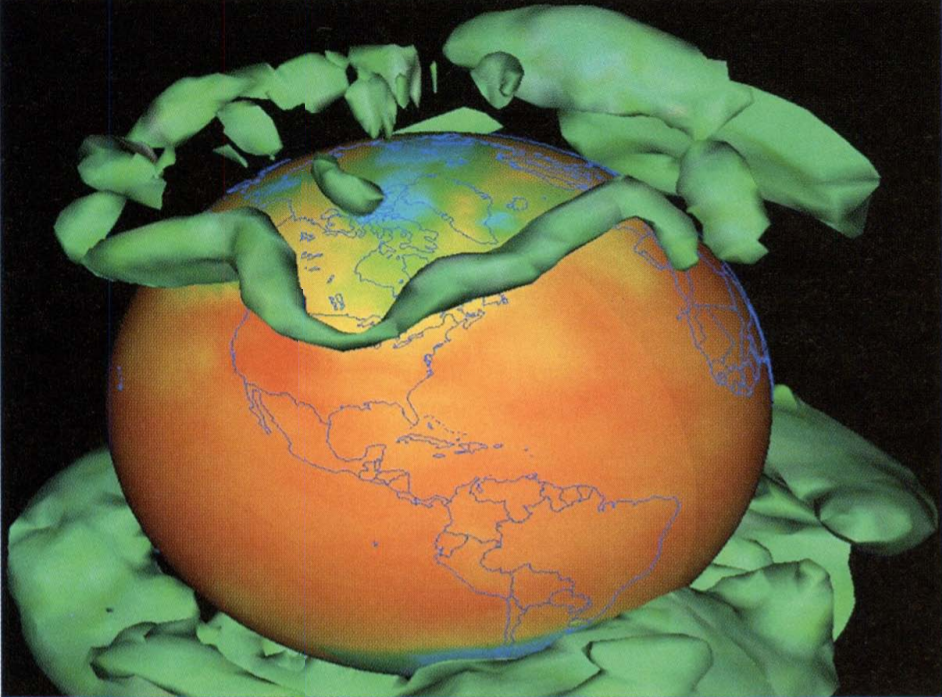
\includegraphics[width=0.7\textwidth]{\FIGDIR/02_01_IVS_Model}
        \caption{Example of upper troposphere winds \cite{rutledge2006nomads}.}
        \label{fig:ExampleOfTroposphereWinds}
    \end{figure}


    \subsection{(R) Mid-Air Collision Prevention}\label{sec:MidairCollisionPrevention}
\paragraph{Idea:} The first fatal mid-air collision occurred in 1912. The occurrence rate increased with technological progress. The \emph{European airspace management} is thoroughly analyzed in \cite{cook2007european}. 

\emph{Mid-Air Collision Situations:} The most common situations when \emph{Mid Air Collision} occurs are:

\begin{enumerate}
    \item \emph{Approach} (airport landing sequence) - the traffic density is increasing with proximity to traffic hub (airport). The aircraft lowers velocity in early approach phase to critical level which significantly reduces maneuverability. The \emph{final approach} phase is most dangerous, because the aircraft is close to the ground prepare to the landing.  
    
    \item \emph{Descent} (decrease of altitude) - the pilot is heading plane down, the dead angle is much greater than in other situations.
    
    \item \emph{Cruise}  (keeping same altitude) - the pilot is  keeping the altitude and heading, the awareness usually decreases significantly in this slight phase. 

    \item \emph{Climb} (increase of altitude) - the pilot is heading plane up, the dead angle is increased significantly. 
\end{enumerate}

\begin{note}
    The \emph{Mid-Air Collision} occurrence is strongly correlating with \emph{traffic density}. Therefore the most of \emph{near miss /collision cases} happens in vicinity of airport. It is expected to elevate the risk of \emph{Mid-Air Collision} by enabling \emph{UAS} into \emph{B, C, D, airports class}  airspace.
\end{note}

\paragraph{Collision Situation Awareness:} The surveillance capability of manned aviation is limited by \emph{pilot`s field of vision} in case of VFR (sec. \ref{sec:VisualFlightRules}) and by \emph{technical limitations} in case of IFR (sec. \ref{sec:InstrumentalFlightRules}). The \emph{surveillance and avoidance} support systems like TCAS (sec. \ref{sec:TCAS}) and ACAS (sec. \ref{sec:ACASX}) can be used as a base of future \emph{DAA} system.

The \emph{UAS} collision situation awareness system is taking the \emph{mid-air} collision prevention to another level, additional functionality needs to be implemented:

\begin{enumerate}
    \item \emph{Intruder trajectory prediction} - anticipate future \emph{intruder actions} based on gathered knowledge. Recognize dangerous actions or triggering situations. The triggering events of future dangerous situations are processed by pilot in manned aviation.
    
    \item \emph{Intruder intersection model} - anticipate future maneuverability and physical properties (turbulence, body size) in intersection model of the intruder and try to estimate an impact area in future. This process is done by pilot in manned aviation. Some supplementary information like \emph{aircraft type} and some properties are provided by surveillance system. The final decision and estimate needs to be automatized in form of impact probability or impact rating. 
    
    \item \emph{Decision making process} - the situation assessment gives an outline of the surrounding space properties, this process is well covered by \emph{surveillance}. The decision making process needs to be flexible and adaptable, but the limited computational resources needs to be taken into account (discretization problem).
\end{enumerate}

\begin{note}
    The \emph{example} of \emph{enclosed operational space} which is necessary for \emph{intruder intersection} detection is given in \cite{welzl1991smallest}.
\end{note}
    \subsection{\secState{R}Weather Impact}\label{sec:WeatherImpact}

\paragraph{Idea:} The \emph{climate} have stable properties over the course of the year. There are observations that climate is shifting in Europe, the periods of sprint/autumn weather are shortening, the periods of summer and winter are prolonging. 

Overall the \emph{European Climate} is getting similar to \emph{North America`s} continental climate. This has severe impact on many aspects of modern society including transportation, specially aviation, emerging UAS industry. 

The key fact is that occurrence of critical weather conditions, like storms or heavy winds is increasing. Along with increasing intensity of these events, the magnitude increases to non-construction mitigable levels.

\paragraph{Transportation Impact:} The \emph{train transportation} is most robust and very infrastructure dependant transportation type. On the other hand, the \emph{aerial transportation} infrastructure is sparse and most of the maneuvering is done in open airspace. 

\emph{Weather Impact} on transportation in general has been introduced by Koetse in study \cite{koetse2009impact}. The \emph{bad weather} situations are well avoidable by \emph{general aviation}. The \emph{general aviation} avoidance capability comes from \emph{high organization} of controlled \emph{airspace}, high grade of surveillance equipment (weather radar).

The situation with \emph{UAS} systems is different, they usually have more delicate construction and significantly smaller take off weight. The \emph{weather} could be even harsher on the lower altitudes. The \emph{implementation} of \emph{weather avoidance} is necessary for \emph{safe UAS operations} in non-controlled airspace. The \emph{UAS operations} can stick to existing \emph{existing} weather avoidance approaches in controlled airspace. 

The \emph{challenge} to avoid weather situations is similar to geo-fencing problem on low altitudes. The \emph{serious weather case} can be encapsulated into protected area with some \emph{altitude limitations}.

\paragraph{Weather avoidance:} \emph{Weather-based} preemptive planning have been introduced into manned aviation in 2015 \cite{yamashita2015climate}. There is an  global approach to weather avoidance. Meaning there is one global \emph{weather model}. Similar impact on every \emph{controlled airspace} attendant. This impact model needs to be refined for various \emph{aircraft classes}.  

\begin{note}
    The \emph{UAS classes} are summarized in (tab. \ref{tab:smallDroneClessesAccordingtoEASA}), the \emph{separation minima} is specified in (tab. \ref{tab:proposedseparationMinimaforUAS}). This needs to be accounted in weather impact calculation. 
    
    The \emph{separation minima} is also accounted for \emph{weather} separation. The \emph{UAS} must keep minimal distance to \emph{dangerous weather condition}.
    
    The radius and impact zone of \emph{dangerous weather condition} is evaluated in relation to \emph{UAS} class, the 5 kg machine is more impacted than 150 kg machine or \emph{autonomous personal transportation}.
\end{note}
    
\emph{Severe Weather Condition Detection Capabilities} for current level of standard aviation equipment have been reviewed in \cite{smith2016multi}. The capability is sufficient for medium scale \emph{UAS} (25 kg). The \emph{numeric models} for \emph{local airspace cluster} can have precision up to one cubic meter of air. The precision of \emph{numeric prediction} is depending \emph{weather stations} density and equipment precision.

The \emph{dynamic} routing of \emph{aircraft} (manned aviation) have been outlined in Balaban et. al. \cite{balaban2017dynamic}. The operational space is separated into \emph{altitude layers} where each layer is separated into homogeneous euclidean grid cells. Each cell (fig. \ref{fig:localizedWeatherModelExample}) has evaluation of \emph{relative humidity} (fig. \ref{fig:humidityRelativeLocalizedExample}), \emph{temperature}, \emph{wind velocity and heading} (fig.\ref{fig:localizedWindVectorsExample}). There is possible to make an prediction and route all aircraft in advance. The scaling challenge remains also for this approach. 

\begin{figure}[H]
	\centering
	\begin{subfigure}{0.45\textwidth}
		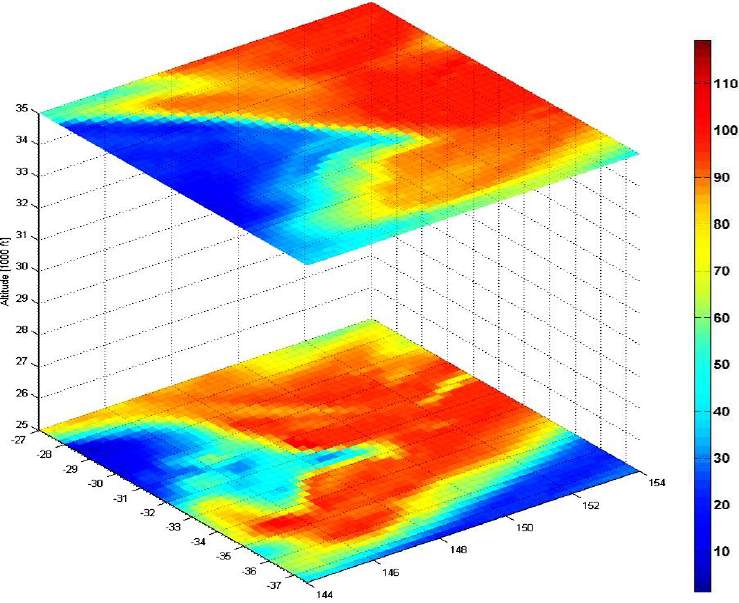
\includegraphics[width=\textwidth]{\FIGDIR/02_03_RelativeHumidity}
		\caption{Relative Humidity.} 
		\label{fig:humidityRelativeLocalizedExample}
	\end{subfigure}
	\vspace{1em} 
	\begin{subfigure}{0.45\textwidth} % width of right subfigure
		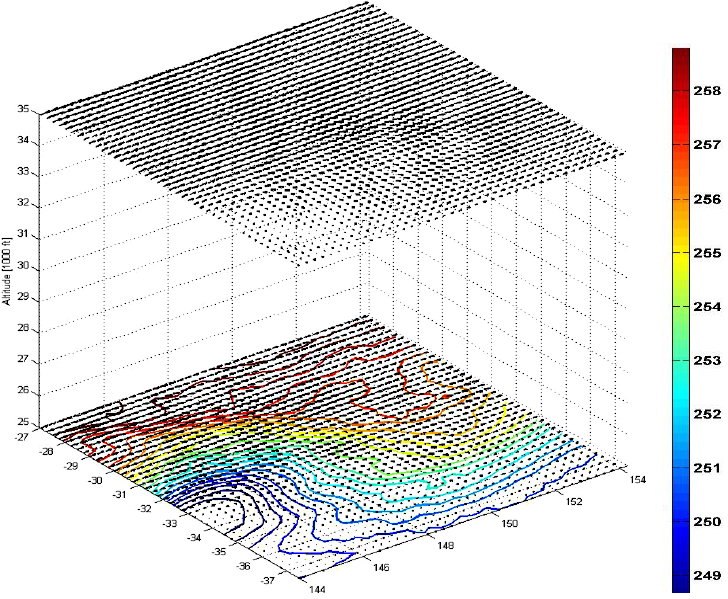
\includegraphics[width=\textwidth]{\FIGDIR/02_04_WindTemperature}
		\caption{Localized Wind Vectors.} % subcaption
		\label{fig:localizedWindVectorsExample}
	\end{subfigure}
	\caption{Localized Weather Model \cite{balaban2017dynamic}.} % caption for whole figure
	\label{fig:localizedWeatherModelExample}
\end{figure}
    
\paragraph{Localized Weather Impact Example:} An \emph{Icing Risk} in localized environment have been predicted based on numerical model \cite{thompson2017numerical}. It is shown that icing can be prevented by \emph{planned} and \emph{reactive} avoidance. The prevention can be done by placing hard or soft constraint into an environment. 

    
\paragraph{Weather Models:} \emph{Weather Models} can be extracted from \emph{Climate and weather model archive at the National Oceanic and Atmospheric Administration} \cite{rutledge2006nomads}. There is an example of troposphere winds (0 - 60 000 feet AMSL) (fig. \ref{fig:ExampleOfTroposphereWinds}) which can be useful in fuel efficient route planning. 
    
\begin{figure}[H]
    \centering
    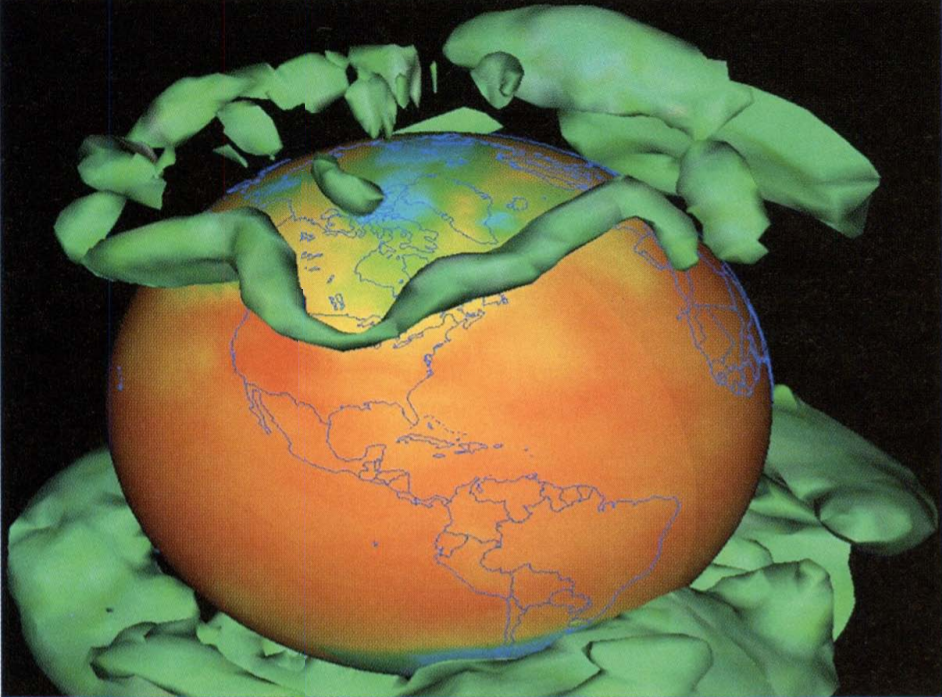
\includegraphics[width=0.7\textwidth]{\FIGDIR/02_01_IVS_Model}
    \caption{Example of upper troposphere winds \cite{rutledge2006nomads}.}
    \label{fig:ExampleOfTroposphereWinds}
\end{figure}
    %Functional decomposition removed
    %\section{(W) UTM Functional Decomposition}\label{sec:UTMFunctionaalDecomposition}
\begin{itemize}
    \item general thinking, approach 
    \item notification run
    \item resolution run
\end{itemize}

\subsection{(W) Information Exchange Principles}\label{sec:InformationExchangePrinciples}
\begin{itemize}
    \item Information Exchange schematics in general, describe data flow and actors
\end{itemize}

\subsubsection{ Collision Case}\label{sec:CollisionCase}
\begin{itemize}
    \item what collision case contains and how is calculated
    \item define conditions and role prioritization
    \item define blank spaces in VFR procedures 
\end{itemize}

\subsubsection{ Weather Case}\label{sec:WeatherCase}
\begin{itemize}
    \item This section needs to be discussed with subject matter expert.
\end{itemize}

\subsection{(W) Resolution Advisories}\label{sec:ResolutionAdvisiories}
\begin{itemize}
    \item just describe the resolution format from ATM
    \item discuss manned/unmanned interaction and reaction delays, reaction uncertainity, etc ...
\end{itemize}
\subsubsection{Movement Restriction}\label{sec:MovementRestriction}
\subsubsection{Convergence/Divergence}\label{sec:ConvergenceDivergence}

    

	
%% This adds a line for the Bibliography in the Table of Contents.
\addcontentsline{toc}{chapter}{Bibliography}
%% *** Set the bibliography style. ***
%% (change according to your preference/requirements)
%\bibliographystyle{plain}
%% *** Set the bibliography file. ***
%% ("thesis.bib" by default; change as needed)
\bibliography{thesis}

%% *** NOTE ***
%% If you don't use bibliography files, comment out the previous line
%% and use \begin{thebibliography}...\end{thebibliography}.  (In that
%% case, you should probably put the bibliography in a separate file and
%% `\include' or `\input' it here).

\end{document}
